%%%%%%%%%%%%%%%%%%%%%%%%%%%%%%%%%%%%%%%%%%%%%%%%%%%%%%%%%%%%%%%%%%%%%%%%%%
%%%%%%%%%%%%%%%%%%%%%%%%%%%%%%%%%%%%%%%%%%%%%%%%%%%%%%%%%%%%%%%%%%%%%%%%%%
\clearpage{}
\section{Determination of signal yield from a fit to the tagjet pair invariant mass $m_{jj}$ distribution}
\label{sec:mjj_fit}
We extract the electroweak W+2jets signal yield from an unbinned maximum
likelihood fit to the tag jet pair invariant mass $m_{jj}$ distribution in the data.

\subsection{Modeling Individual Processes}
We employ a paramatric function to model both signal and background processes. Only high side of tagjet pair invariant mass $m_{jj} > $ 1000 GeV is used in the fit to avoid bad modeling of signal and background shapes. The two parameter power law function is:
\begin{equation}
   \mathcal{F} =  \frac{1.0}{m_{jj}^{a_{0} + a_{1}log(m_{jj}/8000)}}
\end{equation}
where $a_{0}$ and $a_{1}$ paramters obtained from the fit to the Monte Carlo.
This function is a good description of both signal and background shapes.

\subsubsection{W+jets Background}
\label{sec:wjetsShape}
In Figs.~\ref{fig:WpJFit_Dijet},~\ref{fig:WpJFit_Dijet_Pull}, we show the result of an unbinned maximum likelihood fit to the MC distributions. As can be seen, there is a good agreement between projection and the simulation.

W+jets shape paramters are float during the fit to data because of inadequate statistics in the W+jets MC sample and the overall poor agreement between W+jets MC and data distibutions.

W+jets normalization scale factor is obtained from the fitting to BDT output distribution by applying reverse BDT cut($<$ 0.1). In this W+jets dominant region, we fix other background processes(Top, Z+Jets and Diboson) contribution to MC prediction. The W+jets normalization scale factor fit result can be found in Table~\ref{tab:bdtfitcontrol}. Then we apply this W+jets normalization scale factor in the tagjet pair invariant mass $m_{jj}$ fit.  

\begin{figure}
\begin{center}
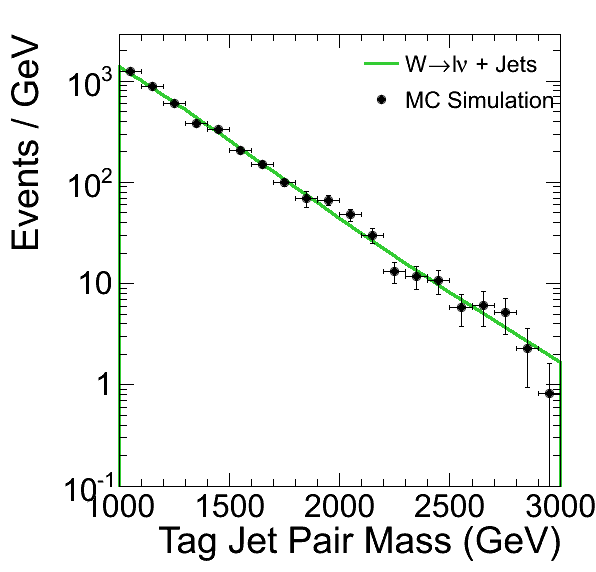
\includegraphics[width=0.45\textwidth]{figs/wpj/EWKW2jetstagjetmjj_WpJ_muon_Model_12_Validate.png}
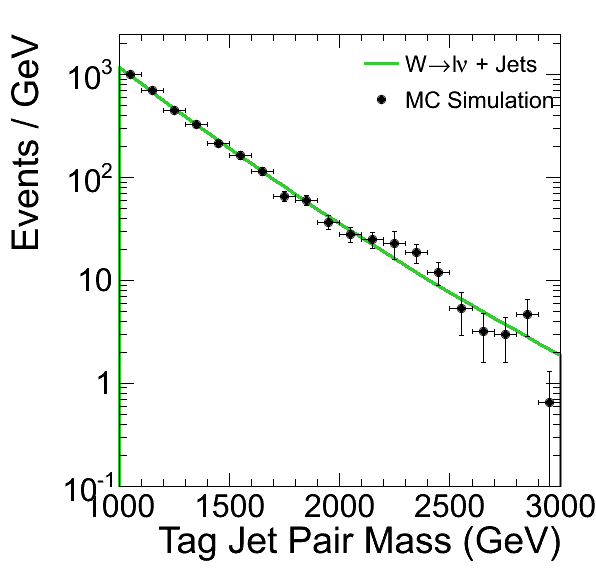
\includegraphics[width=0.45\textwidth]{figs/wpj/EWKW2jetstagjetmjj_WpJ_electron_Model_12_Validate.png}
\end{center}
\caption{\label{fig:WpJFit} W+jets tagjet pair mass $m_{jj}$ shape:
Projection of a fit to the W+jets MC for muons (left) and electrons (right).}
\label{fig:WpJFit_Dijet}
\end{figure}

\begin{figure}
\begin{center}
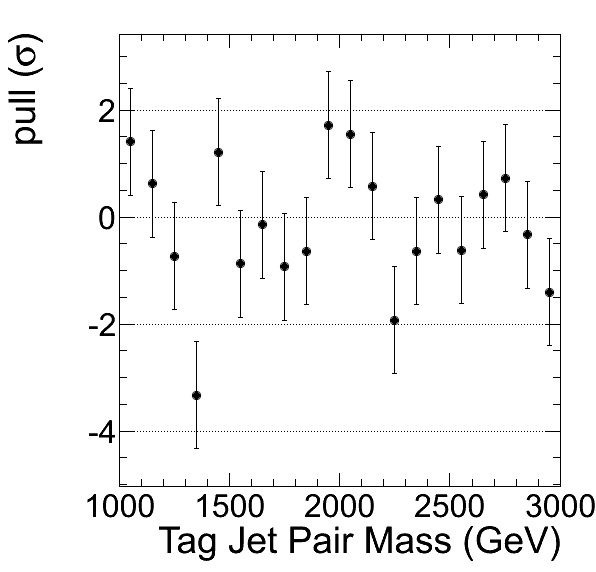
\includegraphics[width=0.45\textwidth]{figs/wpj/EWKW2jetstagjetmjj_WpJ_muon_Model_12_Validate_pull.png}
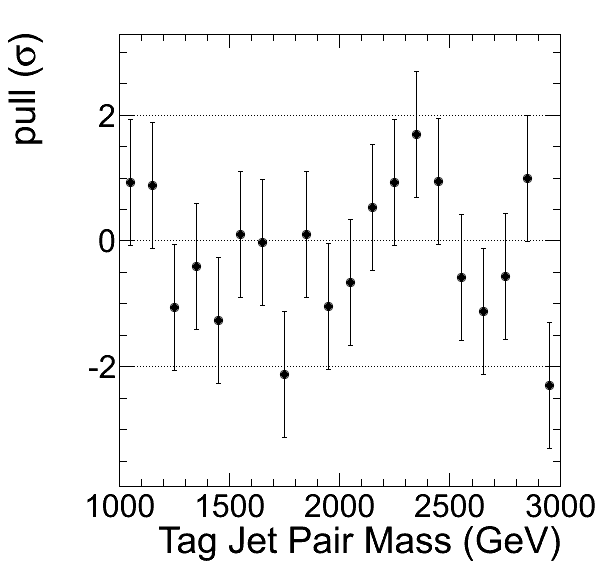
\includegraphics[width=0.45\textwidth]{figs/wpj/EWKW2jetstagjetmjj_WpJ_electron_Model_12_Validate_pull.png}
\end{center}
\caption{\label{fig:WpJFit} W+jets tagjet pair mass $m_{jj}$ shape:
Pull distribution of a fit to the W+jets MC for muons (left) and electrons (right).}
\label{fig:WpJFit_Dijet_Pull}
\end{figure}

\begin{table}[htb]
\centering
\begin{tabular}{|c|c|c|}
\hline
Channels &  Muons & Electrons \\ \hline
W+jets normalization scale factor fit result & 0.859 $\pm$ 0.025(stat) & 0.930 $\pm$ 0.027(stat)\\ \hline
\end{tabular}
\caption{W+jets normalization scale factor from the reverse BDT output distribution fit}
\label{tab:bdtfitcontrol}
\end{table}

%\subsubsection{Matrix Element - Parton Shower Matching And Factorization/Renormalization Scale Uncertainties}
%The potential V+Jets shape variations due to the choice of ME-PS Matching and Factorization/Renormalization scales are accounted for using the corresponding samples (described in section~\ref{sec:wjetsShapeMatchingQ2}). Due to limited statistic of ME-PS Matching and Factorization/Renormalization scales systematic samples, we don't use these samples. In oder to account for mismodeling of Wjets background shape, we float the Wjets shape parameter in the fit.

\subsubsection{Diboson and Drell-Yan Background}
The diboson background is a combination of the WW, WZ and ZZ processes (combined in MC based on their expected cross sections). 
The results of the parametric shape fit to the simulation are displayed in Figs.~\ref{fig:dibosonFit_Dijet},~\ref{fig:dibosonFit_Dijet_Pull}. The diboson shape parameters are fixed to MC and normalization is fixed to NLO cross section predictions in the fit to data.

Drell-Yan shape paramters and normalization are treated the same as the diboson background. The parametric shape fit of Drell-Yan process are displayed in Figs.~\ref{fig:zjetsFit_Dijet},~\ref{fig:zjetsFit_Dijet_Pull}.

\begin{figure}
\begin{center}
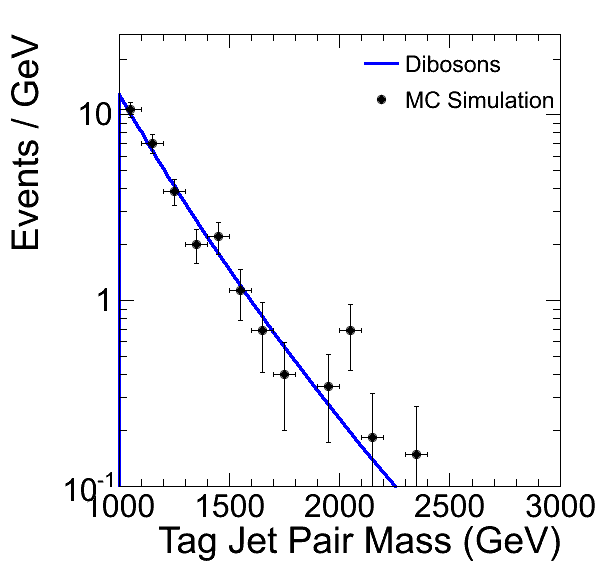
\includegraphics[width=0.45\textwidth]{figs/wpj/EWKW2jetstagjetmjj_diboson_muon_Model_12_Validate.png}
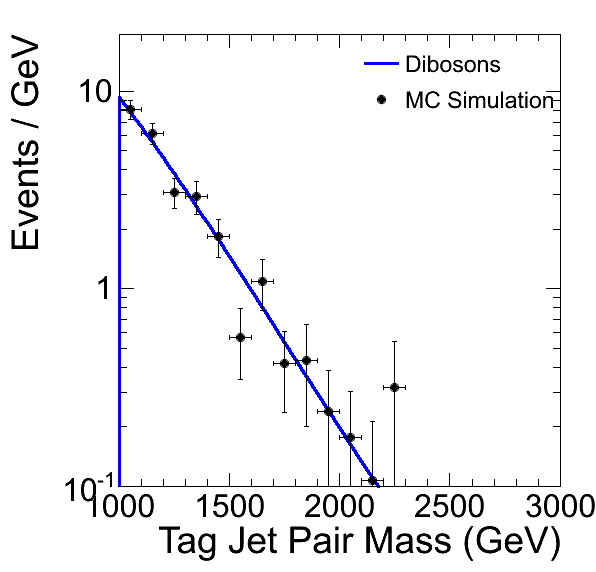
\includegraphics[width=0.45\textwidth]{figs/wpj/EWKW2jetstagjetmjj_diboson_electron_Model_12_Validate.png}
\end{center}
\caption{\label{fig:dibosonFit} Diboson tagjet pair mass $m_{jj}$ shape: projection of a fit to the diboson MC for muons (left) and electrons (right).}
\label{fig:dibosonFit_Dijet}
\end{figure}

\begin{figure}
\begin{center}
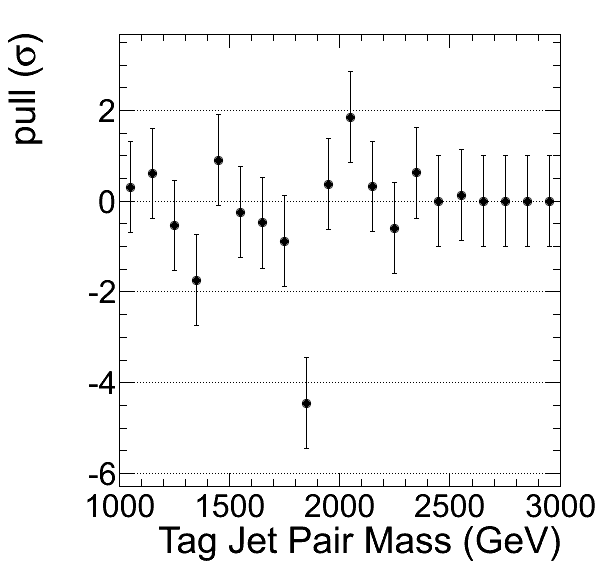
\includegraphics[width=0.45\textwidth]{figs/wpj/EWKW2jetstagjetmjj_diboson_muon_Model_12_Validate_pull.png}
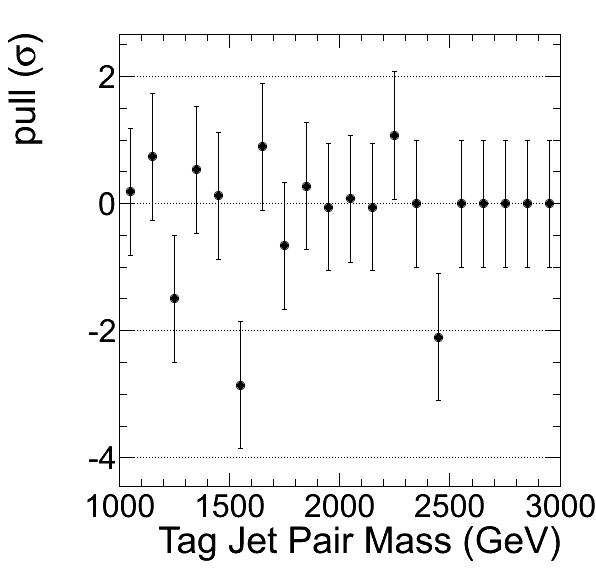
\includegraphics[width=0.45\textwidth]{figs/wpj/EWKW2jetstagjetmjj_diboson_electron_Model_12_Validate_pull.png}
\end{center}
\caption{\label{fig:dibosonFit} Diboson tagjet pair mass $m_{jj}$ shape: Pull distribution of a fit to the diboson MC for muons (left) and electrons (right).}
\label{fig:dibosonFit_Dijet_Pull}
\end{figure}

\begin{figure}
\begin{center}
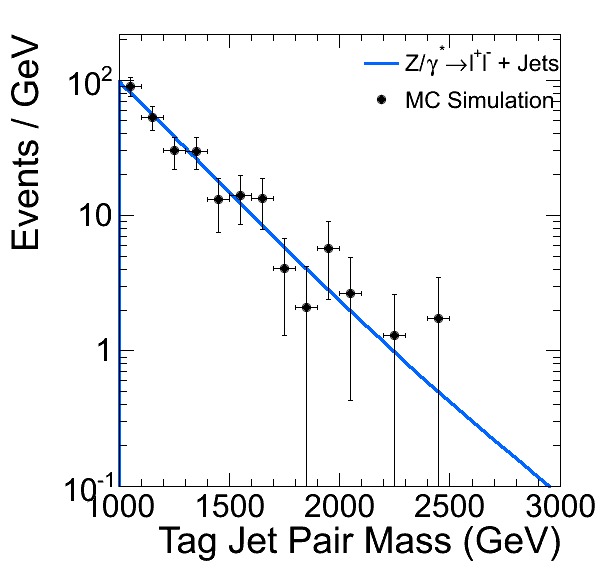
\includegraphics[width=0.45\textwidth]{figs/wpj/EWKW2jetstagjetmjj_ZpJ_muon_Model_12_Validate.png}
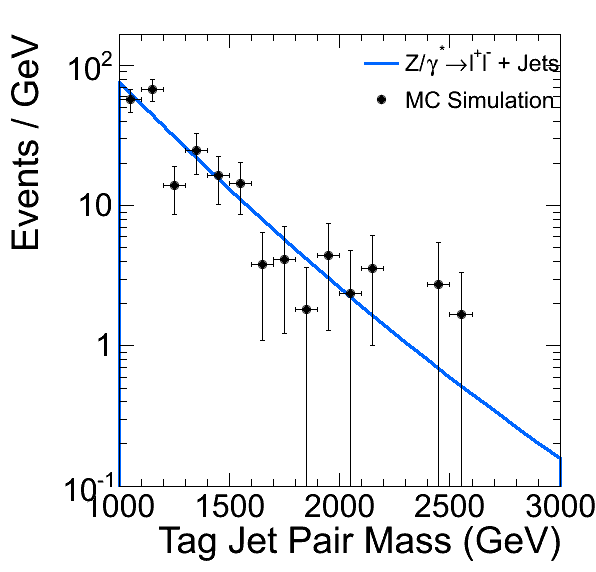
\includegraphics[width=0.45\textwidth]{figs/wpj/EWKW2jetstagjetmjj_ZpJ_electron_Model_12_Validate.png}
\end{center}
\caption{\label{fig:zjetFit} Drell-Yan tagjet pair mass $m_{jj}$ shape: projection of a fit to the Drell-Yan MC for muons (left) and electrons (right).}
\label{fig:zjetsFit_Dijet}
\end{figure}

\begin{figure}
\begin{center}
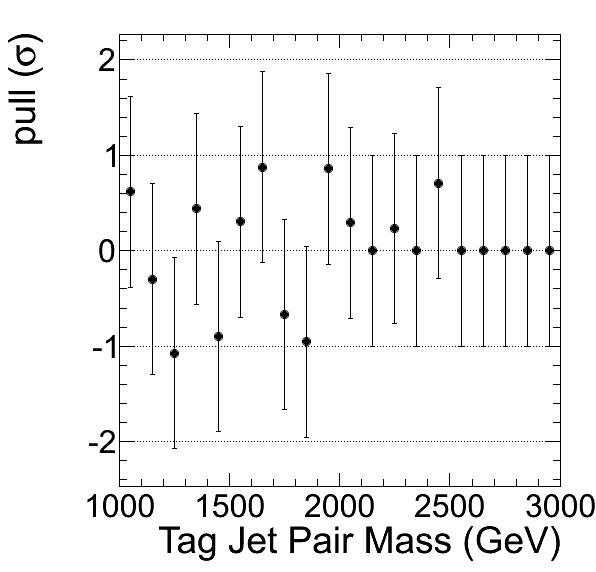
\includegraphics[width=0.45\textwidth]{figs/wpj/EWKW2jetstagjetmjj_ZpJ_muon_Model_12_Validate_pull.png}
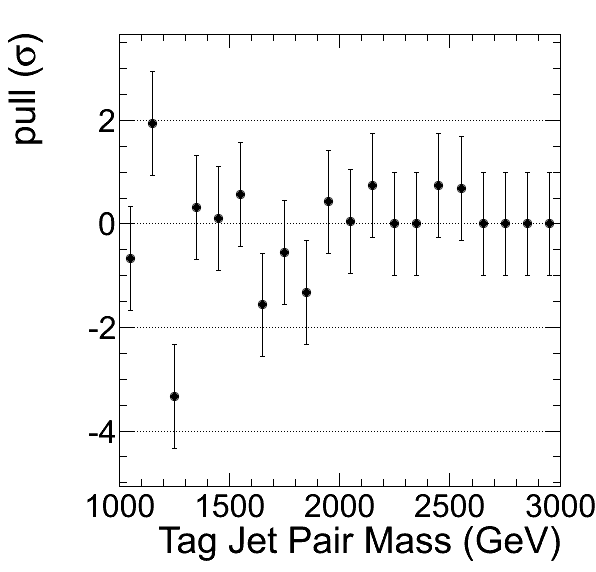
\includegraphics[width=0.45\textwidth]{figs/wpj/EWKW2jetstagjetmjj_ZpJ_electron_Model_12_Validate_pull.png}
\end{center}
\caption{\label{fig:zjetFit} Drell-Yan tagjet pair mass $m_{jj}$ shape: Pull distribution of a fit to the Drell-Yan MC for muons (left) and electrons (right).}
\label{fig:zjetsFit_Dijet_Pull}
\end{figure}

\subsubsection{Top Background}
The top background is a combination of \ttbar\ and single top processes with the MC samples combined based on the expected cross sections. 
The shape parameters are obtained from the simulation (Figs.~\ref{fig:topFit_Dijet},~\ref{fig:topFit_Dijet_Pull}) are fixed during the fit. A Guassisain constraint(7\%) on the Top background normalization is applied in the fit.

%We also use other ttbar samples with different generators(1. aMC@NLO+Herwig 2. Powheg+Pythia) to account for the ttbar shape systematic uncertainty(Details in section~\ref{sec:ttbar_resulved}).

\begin{figure}
\begin{center}
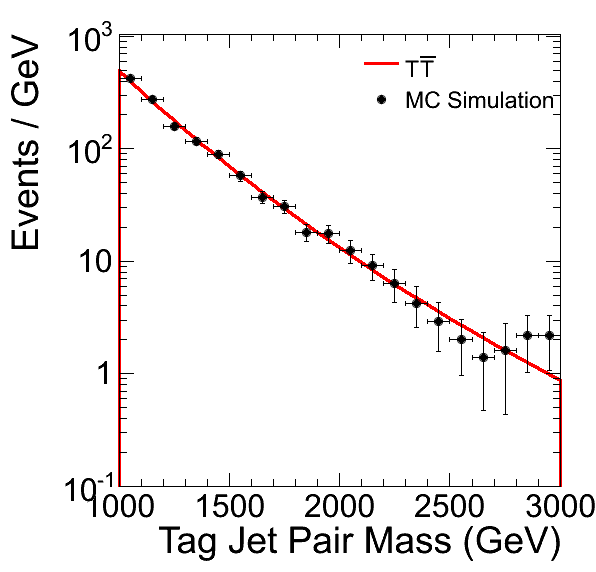
\includegraphics[width=0.45\textwidth]{figs/wpj/EWKW2jetstagjetmjj_top_muon_Model_12_Validate.png}
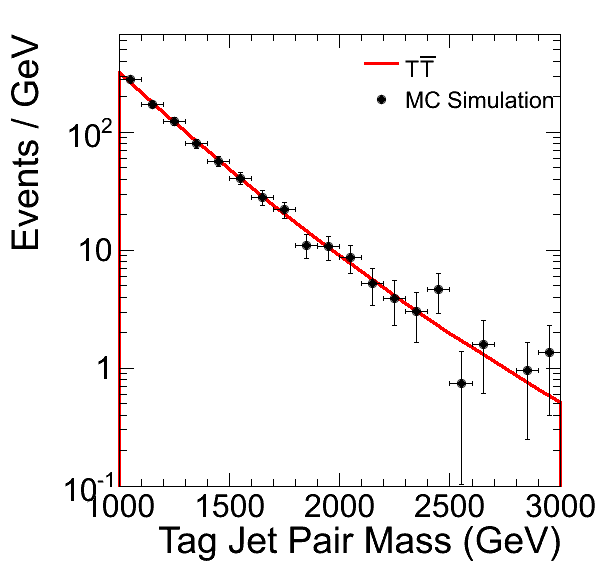
\includegraphics[width=0.45\textwidth]{figs/wpj/EWKW2jetstagjetmjj_top_electron_Model_12_Validate.png}
\end{center}
\caption{\label{fig:topFit} Top tagjet pair mass  $m_{jj}$ shape: projection of a fit to the top MC for muons (left) and electrons (right).}
\label{fig:topFit_Dijet}
\end{figure}

\begin{figure}
\begin{center}
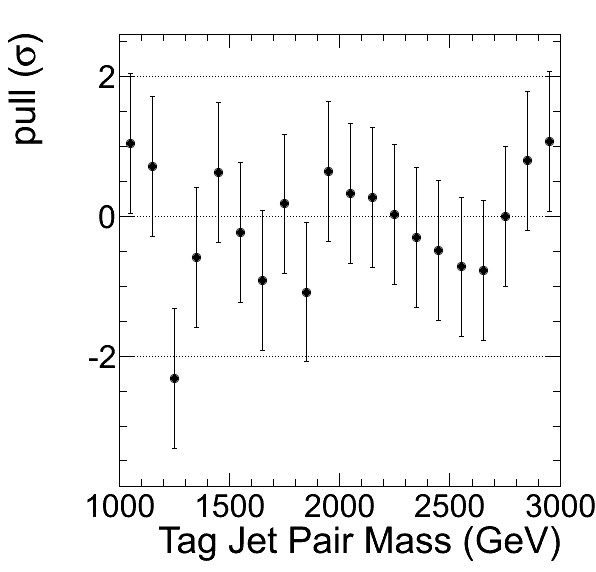
\includegraphics[width=0.45\textwidth]{figs/wpj/EWKW2jetstagjetmjj_top_muon_Model_12_Validate_pull.png}
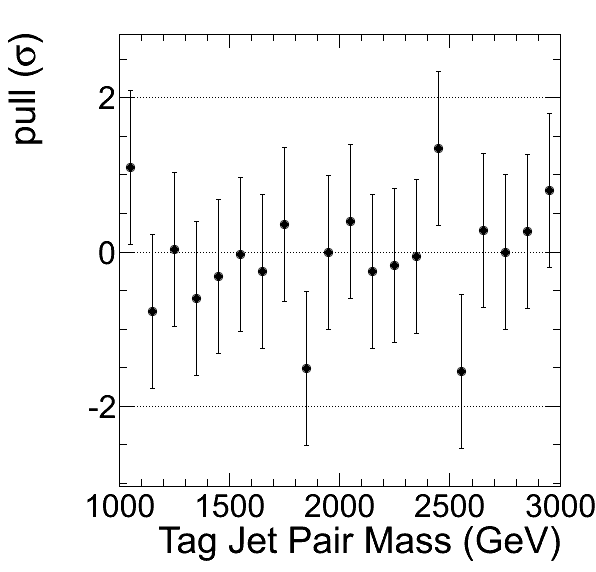
\includegraphics[width=0.45\textwidth]{figs/wpj/EWKW2jetstagjetmjj_top_electron_Model_12_Validate_pull.png}
\end{center}
\caption{\label{fig:topFit} Top tagjet pair mass  $m_{jj}$ shape: Pull distribution of a fit to the top MC for muons (left) and electrons (right).}
\label{fig:topFit_Dijet_Pull}
\end{figure}

\subsubsection{QCD Background}
The electron data events contain a significant contribution from multijet processes. 
A thorough treatment of the QCD background is presented in Section~\ref{sec:qcd}. The shape parameters of the same function are shown in Figs.~\ref{fig:QCDFit_Dijet}. In case of muons the multijet contribution is negligible.

\begin{figure}
\begin{center}
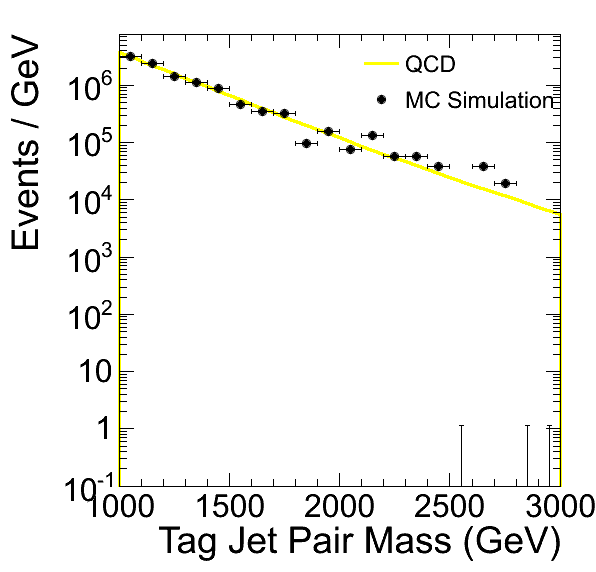
\includegraphics[width=0.45\textwidth]{figs/wpj/EWKW2jetstagjetmjj_QCD_electron_Model_12_Validate.png}
\end{center}
\caption{QCD tagjet pair mass $m_{jj}$ shape in the electron sample: projection of a fit to the QCD data driven shape for electrons.}
\label{fig:QCDFit_Dijet}
\end{figure}

\subsubsection{Electroweak W+2jets Signal}
For the signal shape, the same parametric function is used. The results of the parametric shape fit to the simulation are displayed in Figs.~\ref{fig:ewkw2jets_Dijet},~\ref{fig:ewkw2jets_Dijet_Pull}.

\begin{figure}
\begin{center}
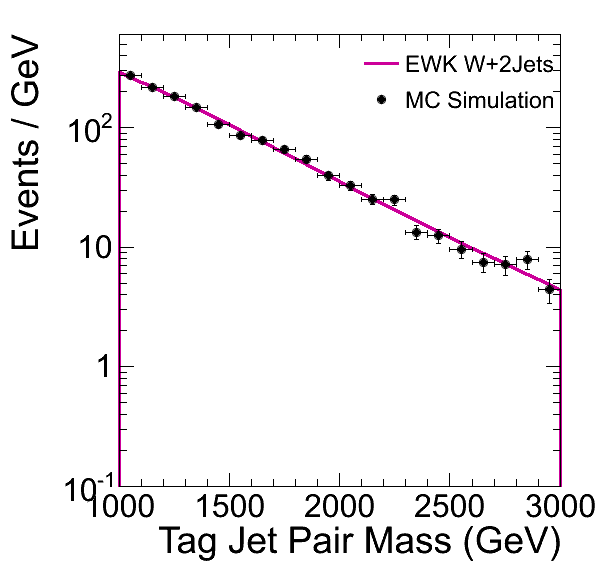
\includegraphics[width=0.45\textwidth]{figs/wpj/EWKW2jetstagjetmjj_EWKW2jets_muon_Model_12_Validate.png}
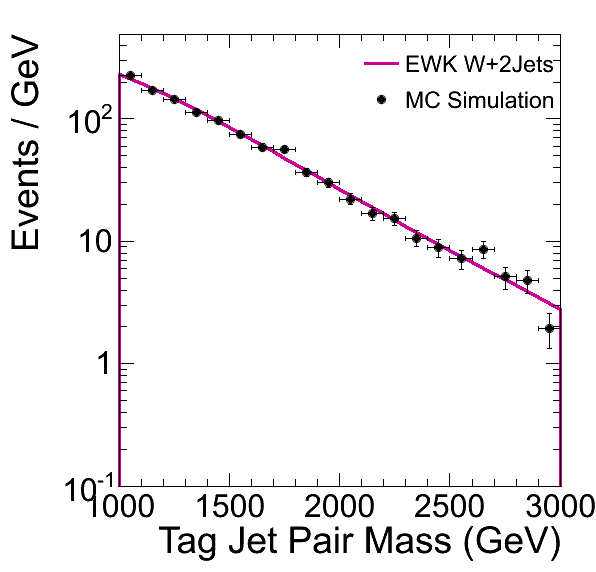
\includegraphics[width=0.45\textwidth]{figs/wpj/EWKW2jetstagjetmjj_EWKW2jets_electron_Model_12_Validate.png}
\end{center}
\caption{\label{fig:topFit} EWK W+2jets tagjet pair mass $m_{jj}$ shape: projection of a fit to the EWK W+2jets MC for muons (left) and electrons (right).}
\label{fig:ewkw2jets_Dijet}
\end{figure}

\begin{figure}
\begin{center}
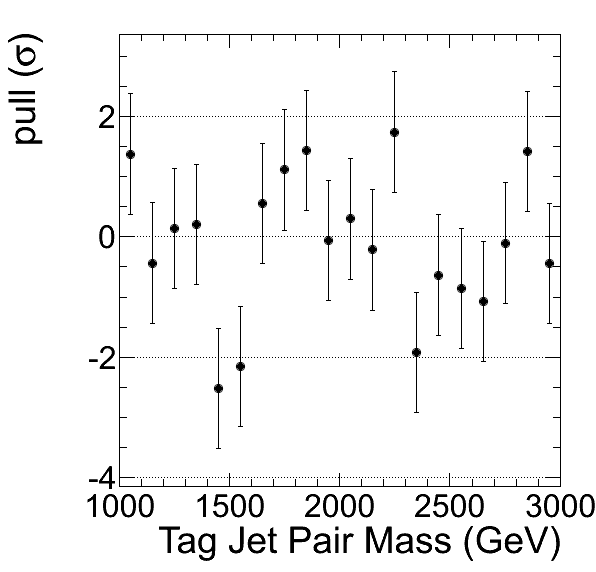
\includegraphics[width=0.45\textwidth]{figs/wpj/EWKW2jetstagjetmjj_EWKW2jets_muon_Model_12_Validate_pull.png}
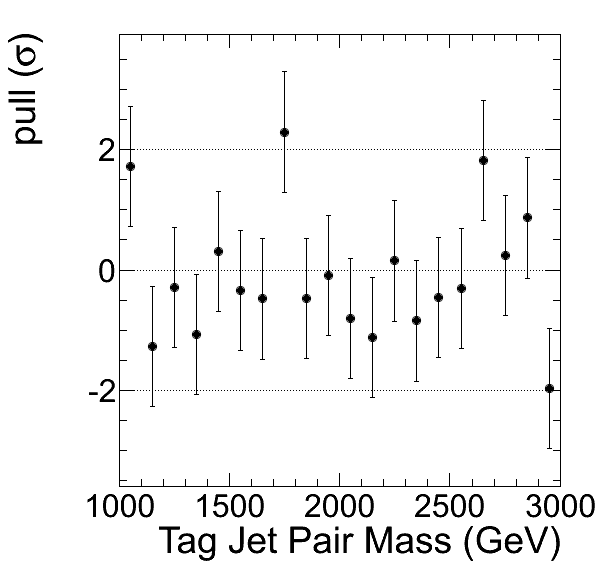
\includegraphics[width=0.45\textwidth]{figs/wpj/EWKW2jetstagjetmjj_EWKW2jets_electron_Model_12_Validate_pull.png}
\end{center}
\caption{\label{fig:topFit} EWK W+2jets tagjet pair mass $m_{jj}$ shape: Pull distribution of a fit to the EWK W+2jets MC for muons (left) and electrons (right).}
\label{fig:ewkw2jets_Dijet_Pull}
\end{figure}

Table~\ref{tab:mjj_shapes_and_normalization} shows how the shape of
each component is determined, and what constraints are applied to fit
for the normalization. 
%while the fit output is summarized in Table~\ref{table:FitTotalsAndComparisons}.  
%The main sources of systematic errors are the uncertainties in the jet energy resolution(JER), jet energy scale(JES), Wjets shape modeling and normalization, as well as ttbar shape moldeing uncertainty.
%%%%%%%%%%%%%%%
\begin{table}[!htbp]
  \begin{center}
 \caption{Determination of the $m_{jj}$ shape and normalization. External constraints are assumed Gaussian.}  
 \label{tab:mjj_shapes_and_normalization} 
 \begin{tabular} {l  c  l}
   \hline \hline
   Process                &    Shape     & External constraint on normalization\\ \hline
   W+jets            &    float   &  Apply scale factor from reverse BDT fit in Table~\ref{tab:bdtfitcontrol}\\
   Diboson                &    fixed to MC    & Fixed to NLO cross section \\ 
   Top                    &    fixed to MC       & Gaussian Constrained: $\pm$ 7\% ~\cite{Kidonakis:2010dk,Kidonakis:2010tc,Kidonakis:2011wy,Kidonakis:2010ux}\\ 
   Drell-Yan    &    fixed to MC       & Fixed to NLO cross section \\%Constrained: (NLO, $m_{ll}>50$~GeV) 3048 pb  $\pm$  4.3\%~\cite{MCFM} \\
   Multijet(Electron channel)               &    data      & Constrained: \MET fit in data $\pm$  50\%  \\\hline 
   \hline
   EWK W+2jets            &   fixed to MC & Unconstrained \\ 
   \hline \hline
 \end{tabular}
\end{center}
\end{table}
%%%%%%%%%%%%%%%%%%%%%%%%%%%%%%%%%%%%%%%%%%%%%%%%%%%%%%%%%%%%
%%%%%%%%%%%%%%%%%%%%%%%%%%%%%%%%%%%%%%%%%%%%%%%%%%%%%%%%%%%%%%%
\subsection{Fit results}
\label{sec:mjj_2jetfit}
The fit results are summarized in Table~\ref{table:FitTotalsAndComparisons} and shown in Figs.~\ref{fig:mjj_2jet_mu},~\ref{fig:mjj_2jet_el}.
%Figs.~\ref{fig:mjj_2jet_mu_btag},~\ref{fig:mjj_2jet_el_btag} for the btagged dijet selection and Figs.~\ref{fig:mJ_mu_boosted},~\ref{fig:mJ_el_boosted} for the boosted events. 
A clear signal from the Standard Model electroweak W+2jets production can be seen. 
%The distribution for the electroweak W+2jets events are 
%consistent with the Standard Model predictions computed up to 
%the next-to-leading order (NLO) in perturbation theory.
%These consistency checks give us confidence in the analysis procedures.
%The fit results are tabulated below.
%%%%%%%%%%%%%%%%%%%%

\underline{Muons Channal Fit Result:}
{\tiny
\input{EWKW2jetsMuons.log}
}

\underline{Electrons Channal Fit Result:}
{\tiny
\input{EWKW2jetsElectrons.log}
}

%%%%%%%%%%%%%%%%%%%%
%%%%%%%%%%%%%%%%%%%%
\begin{figure}[h!]
  {\centering
    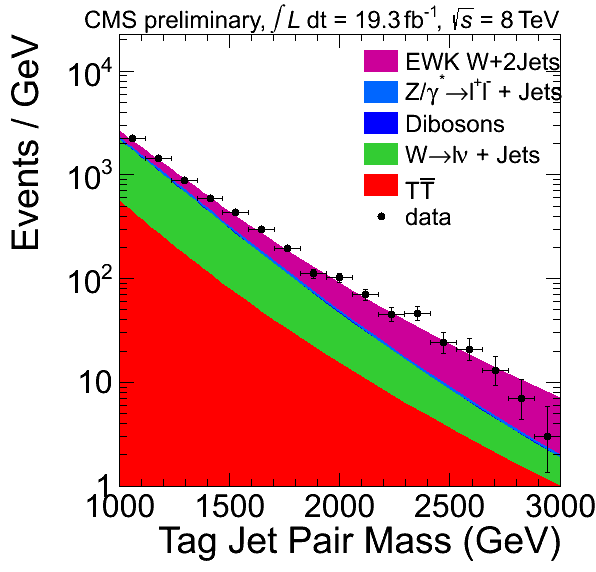
\includegraphics[width=0.49\textwidth]{figs/mjjfit/EWKW2jetstagjetmjj_defaultfit_muon_Stacked.png}
    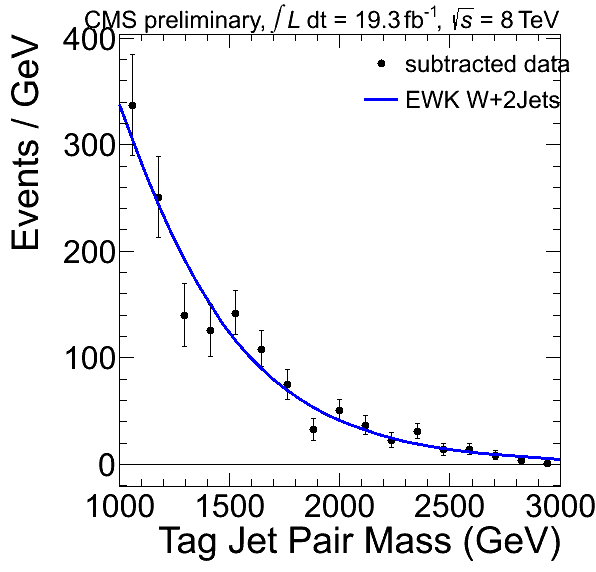
\includegraphics[width=0.49\textwidth]{figs/mjjfit/EWKW2jetstagjetmjj_defaultfit_muon_Subtracted.png}
    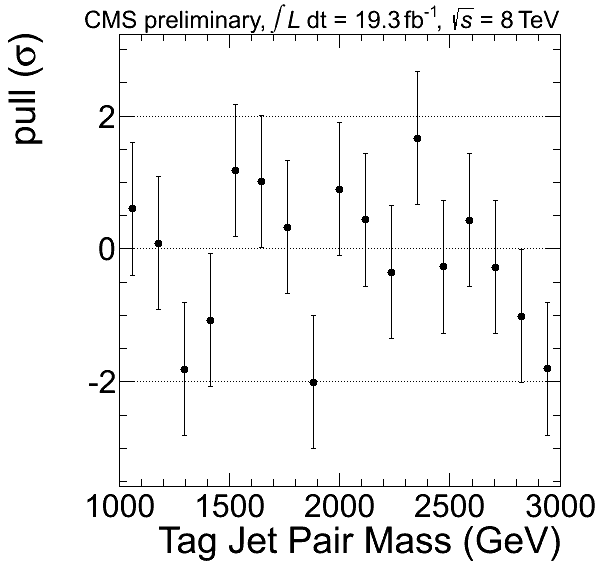
\includegraphics[width=0.49\textwidth]{figs/mjjfit/EWKW2jetstagjetmjj_defaultfit_muon_Pull.png}
    \caption{Distribution of the tagjet pair invariant mass $m_{jj}$ in muon data and fit shapes: 
      (upper left) Signal and background components stacked together, 
      (upper right) Data minus all backgrounds except EWK W+2jets,  
      (lower) Pull distribition of the fit.}
    \label{fig:mjj_2jet_mu}}
\end{figure}
%%%%%%%%%%%%%%%%%%%%
%%%%%%%%%%%%%%%%%%%%
\begin{figure}[h!]
  {\centering
    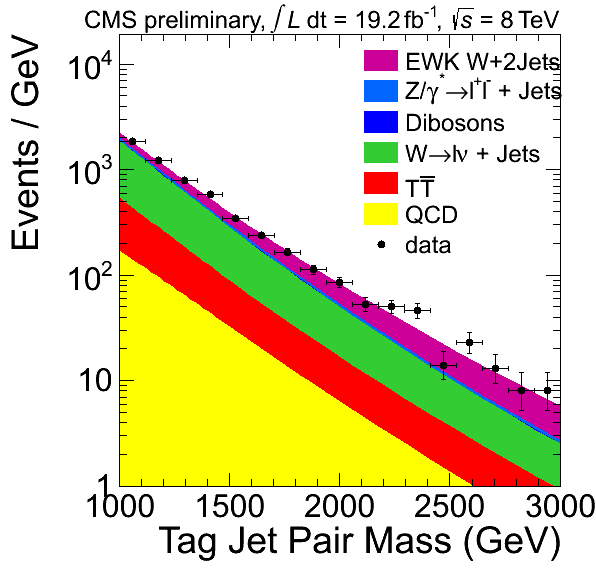
\includegraphics[width=0.49\textwidth]{figs/mjjfit/EWKW2jetstagjetmjj_defaultfit_electron_Stacked.png}
    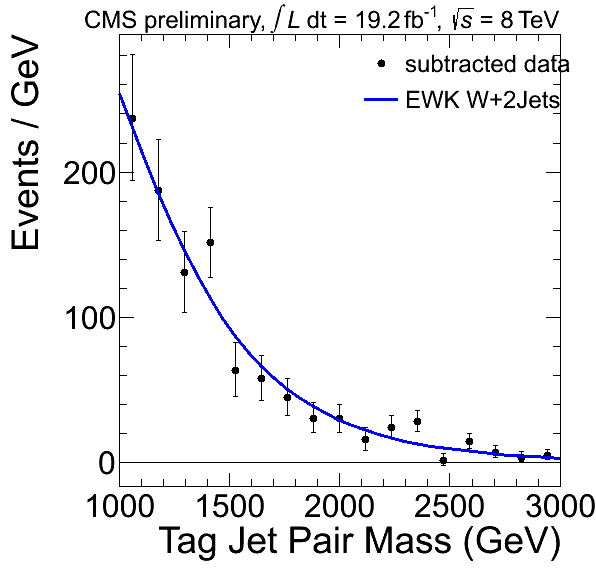
\includegraphics[width=0.49\textwidth]{figs/mjjfit/EWKW2jetstagjetmjj_defaultfit_electron_Subtracted.png}
    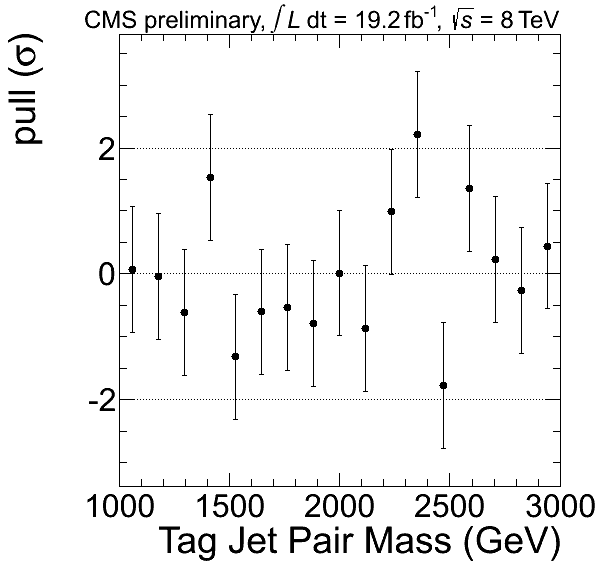
\includegraphics[width=0.49\textwidth]{figs/mjjfit/EWKW2jetstagjetmjj_defaultfit_electron_Pull.png}
    \caption{Distribution of the tagjet pair invariant mass $m_{jj}$ in electron data and fit shapes: 
      (upper left) Signal and background components stacked together, 
      (upper right) Data minus all backgrounds except EWK W+2jets,  
      (lower) Pull distribition of the fit.}
    \label{fig:mjj_2jet_el}}
\end{figure}
%%%%%%%%%%%%%%%%%%%%
%%%%%%%%%%%%%%%
\begin{table}[tbht!]
\begin{center}
\caption{Fractions of the expected yields determined from a likelihood fit to the data}
%the expected event counts and the EWK W+2jets Fraction as well as Error corrected for the fit bias (as described in Section~\ref{sec:FitValidation}.}
 \label{table:FitTotalsAndComparisons}
\vspace{0.5cm}
\scalebox{0.90}{
 \begin{tabular} {l c c c c }
   \hline \hline
Bin            &  \multicolumn{2}{c}{Muons} & \multicolumn{2}{c}{Electrons} \\  
\hline
               & Predicted &   Extracted Fraction     &  Predicted &  Extracted Fraction \\
\hline
EWK W+2jets    & 1392.3 $\pm$ 37.3 & 1.008 $\pm$ 0.082    & 1111.0 $\pm$ 33.3  &  0.942 $\pm$ 0.086 \\
Dibosons       & 29.5 $\pm$ 5.4 & 1.000(fixed)   & 25.4 $\pm$ 5.0   &  1.000(fixed)   \\
Multijet       &  ---   &   ---           &  443.5   &  fixed to \MET fit in data \\
Top            & 1263.2 $\pm$ 35.4   & 0.998 $\pm$ 0.069   & 859.1 $\pm$ 29.3    &   0.994 $\pm$ 0.069\\
W+Jets         & 4143.9 $\pm$ 64.4 &  0.859(fixed see Table~\ref{tab:bdtfitcontrol})   & 3261.9 $\pm$ 57.1  &  0.930(fixed see Table~\ref{tab:bdtfitcontrol}) \\
Z+Jets         & 260.9 $\pm$ 16.2 &  1.000(fixed)   & 218.4 $\pm$ 14.8   &  1.000(fixed) \\
\hline
Total Yields   & ---- & 6518  & ---- & 5621 \\ 
\hline 
%Corrected EWK W+2jets &  1392.3 $\pm$ 37.3 & 1.008 $\pm$ 0.082   & 1111.0 $\pm$ 33.3  &  0.942 $\pm$ 0.086 \\
%\hline 
Data           & ----  & 6514             & ----  &  5614  \\ 
\hline
\end{tabular}}
\end{center}
\end{table}

%\begin{table}[bthp]
%\begin{center}
%\caption{\label{tab:dibosonYield} Electroweak W+2jets signal yields along with corresponding cross-sections, with the statistical contribution and the systematic contribution to the uncertainties broken out. The first uncertainty arises chiefly from statistics the second is from systematic sources.}
%\begin{tabular}{rcc}
%\hline\hline
%& muons & electrons \\
%\hline
%N EWKW2jets               & $$ \\
%$\sigma_{EWKW2jets}$ (pb)      & $$ \\
%\hline\hline
%\end{tabular}
%\end{center}
%\end{table}
%%%%%%%%%%%%%%%
%%%%%%%%%%%%%%%
%%%%%%%%%%%%%%%%%%%%%%%%%%%%%%%%%%%%%%%%%%%%%%%%%%%%%%%%%%%%

%%%%%%%%%%%%%%%
\begin{table}[bthp]
\begin{center}
\caption{\label{tab:SystematicCorrections} EWK W+2jets signal yield, significance(statistic) and fit bias for each channel. The bottom line is the EWK W+2jets yield and error after the correction for the fit bias (as described in Section~\ref{sec:FitValidation}.)}
\label{table:FitCorrectedYields}
\begin{tabular}{rcc}
\hline\hline
Quantity       & muons & electrons \\
\hline
Fit Yield      &  1403.6 $\pm$ 115.3   &  1046.6 $\pm$ 95.6 \\
Significance   &  12.1$\sigma$   & 11.1$\sigma$ \\
Yield Bias     &   -3.3     &  -10.7 \\
Fractional Error Bias & 	0.781     &  0.685  \\
\hline
Corrected fit Yield      &  1400.3 $\pm$ 90.0   &  1035.9 $\pm$ 65.5 \\
\hline
\hline\hline
\end{tabular}
\end{center}
\end{table}
%%%%%%%%%%%%%%%

%%%%%%%%%%%%%%%%%%%%%%%%%%%%%%%%%%%%%%%%%%%%%%%%%%%%%%%%%%%%
%%%%%%%%%%%%%%%%%%%%%%%%%%%%%%%%%%%%%%%%%%%%%%%%%%%%%%%%%%%%
\clearpage
\subsection{Fit Validation and Cross Check}
\label{sec:FitValidation}
We verify that the signal extraction procedure is unbiased and that 
statistical uncertainties reported have good coverage by constructing
and fitting toy datasets. 
%Since our fit procedure is the same in both
%electron and muon channels, we validate and perform a number of cross-checks
%using muons; with the electron results subsequently listed. 
The specific steps are:
\begin{enumerate}
\item Perform the default fit and obtain the expected yields 
(Table~\ref{table:FitTotalsAndComparisons}).
\item Generate toy Monte Carlo for each process from the corresponding MC distributions.
\item Construct 2000 sample datasets. The excpected yield are first smeared by the fit 
errors, with correlations taken into account, by computing the errors in a coordinate frame 
where they are uncorrelated and rotating back (Sec.~\ref{sec:FitValidation_ExpectedEventGeneration}). 
Afterwards, we smear the expected yields by the Poisson Errors.
\item Perform the fit for each sample dataset.
\item Examine the resultant Yields and Pulls.
\end{enumerate}


\subsubsection{Expected Event Generation}
\label{sec:FitValidation_ExpectedEventGeneration}
Due to the constraints imposed by the data, the fitted event yields are strongly correlated
(Sec.~\ref{sec:mjj_2jetfit}). This fact is taken into account 
when smearing the expected values. In short we perform a transformation to 
the coordinate system where the yields are uncorrelated, smear and transform back. Specifically,
for each toy dataset we:
\begin{enumerate}
\item Diagonalize the Covariance Matrix ($\Sigma$) obtained from the original fit to the 
data (Sec.~\ref{sec:mjj_2jetfit}). I.e. find $M$ such that $M\Sigma M^{-1}$ is 
diagonal (Rows of $M$ are in fact the eigenvectors of $\Sigma$).
\item Produce the errors ($z_i$) in a frame where there is no correlation between the fitted 
'yields' (i.e. in a frame where the Covariance Matrix is diagonal). Namely, $z_i$ are randomly 
selected from a Gaussian distribution with $\sigma_i^2=(M\Sigma M^{-1})_{ii}$ and mean$=0$.
\item Transform back to the orignal frame and obtain the yields ($x_i$) smeared by the fit error: 
$x_i=\mu_i+(M^{-1}Z)_i$, where $\mu$ is the expected value from the default fit.
\item Poisson-smear $x_i$ and generate the dataset with the obtained values.
\item Perform the fit.
\end{enumerate}
This procedure is designed to sample in the vicinity of the fit result, while taking the likelihood of a particular configuration into account. The resultant Yield and Pull distributions are examined to see if they are Gaussian, whether there is any bias in the yield and how close the pull $\sigma$ is to unity.


\subsubsection{Fit Configuration Validation}
The first step is to determine if there is any inherent bias in the fit. As such we use the yield and shape parameter values returned by the fit to generate toy datasets and refit them. Because only the signal and ttbar yields are not fixed during the fit, only signal and ttbar yields are validated 
 by using Toy MC method.
The results are shown in Figs.~\ref{fig:Validation_mu_Standard},~\ref{fig:Validation_el_Standard}. %Figs.~\ref{fig:Validation_mu_Btag},~\ref{fig:Validation_el_Btag} for the btagged dijet configuration and in Figs.~\ref{fig:Validation_mu_Boosted},~\ref{fig:Validation_el_Boosted} for the boosted case.

%%%%%%%%%%%%%%%%%%%%%%%%%
%%%%%%%
\begin{figure}[h!] {\centering
\unitlength=0.33\linewidth
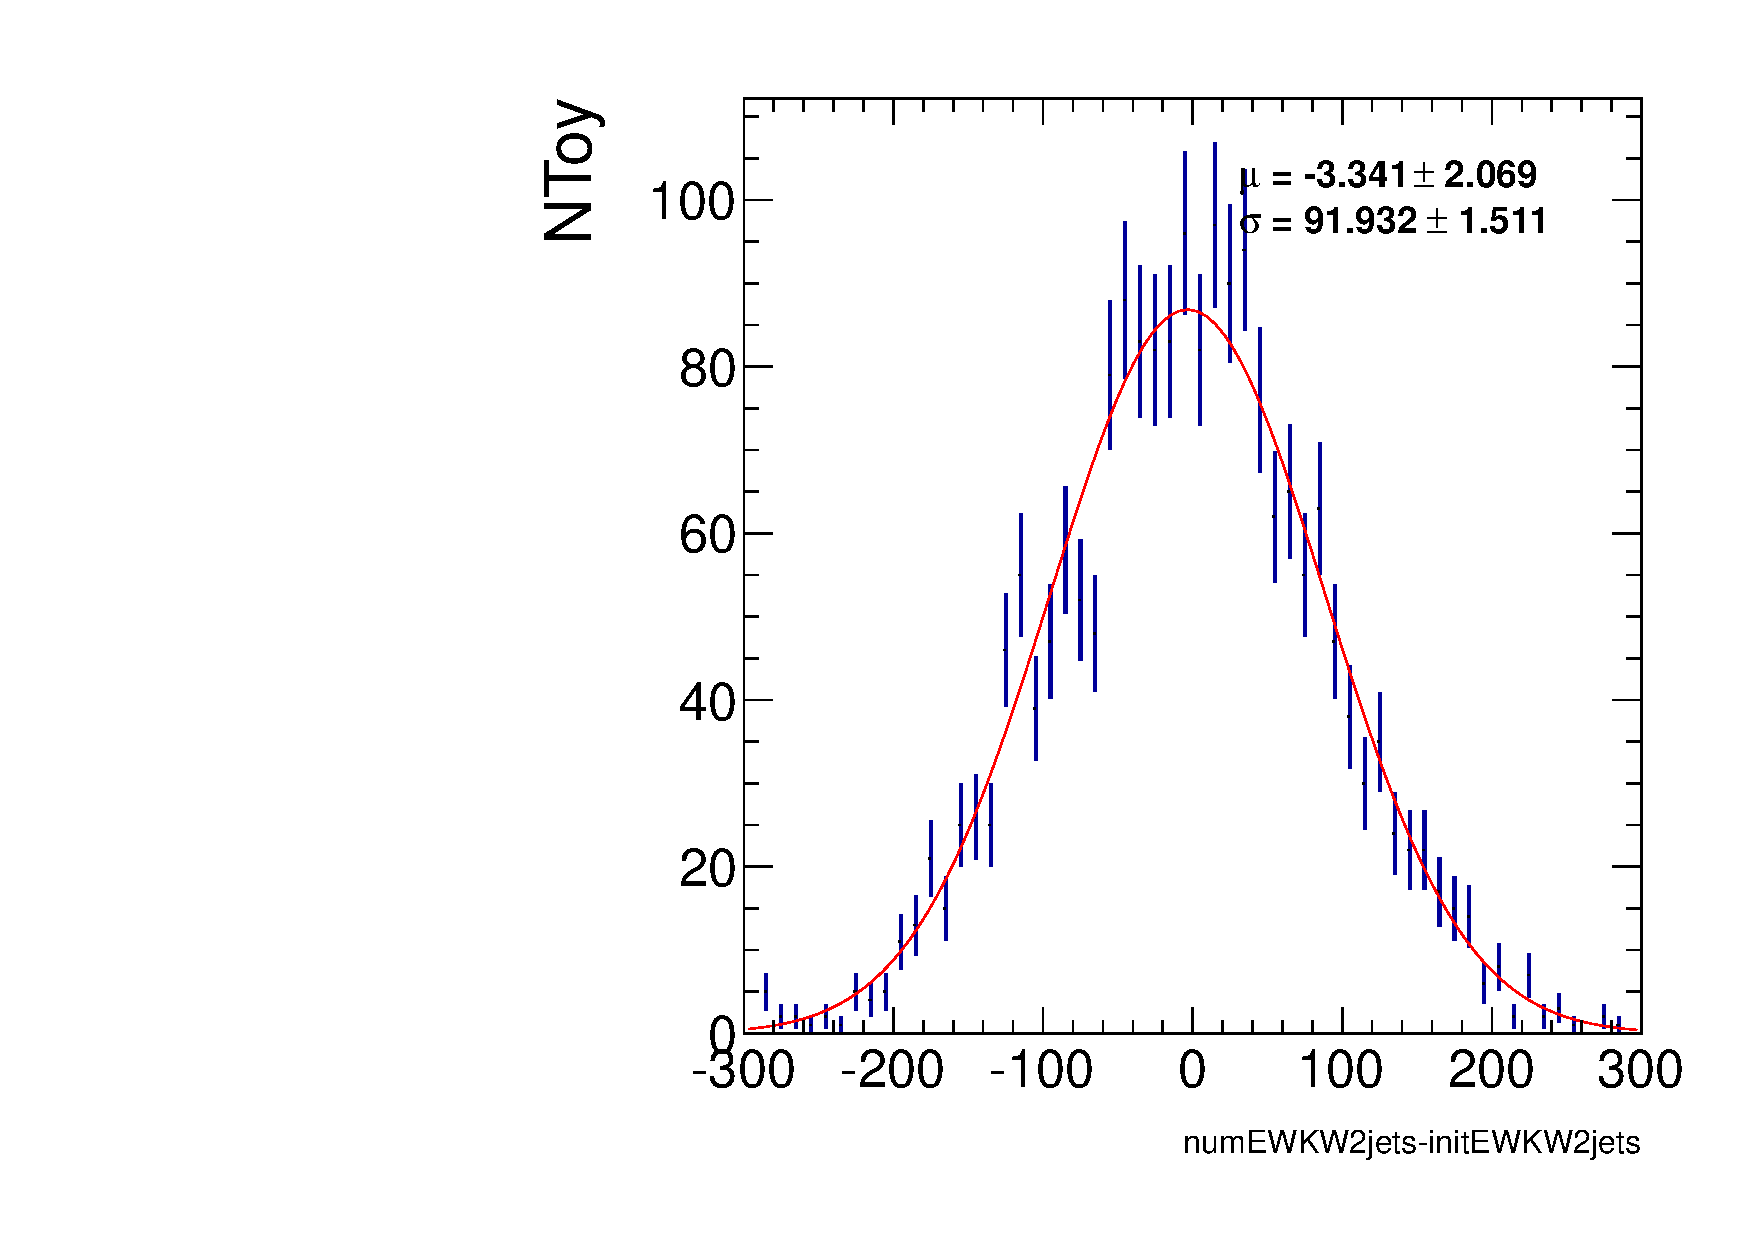
\includegraphics[width=0.48\textwidth]{figs/validation/mu_numEWKW2jets_initEWKW2jets_EWKW2jetsbiasplot_pulldistribution.pdf}
\put(-0.80,0.0){(a)}
\unitlength=0.33\linewidth
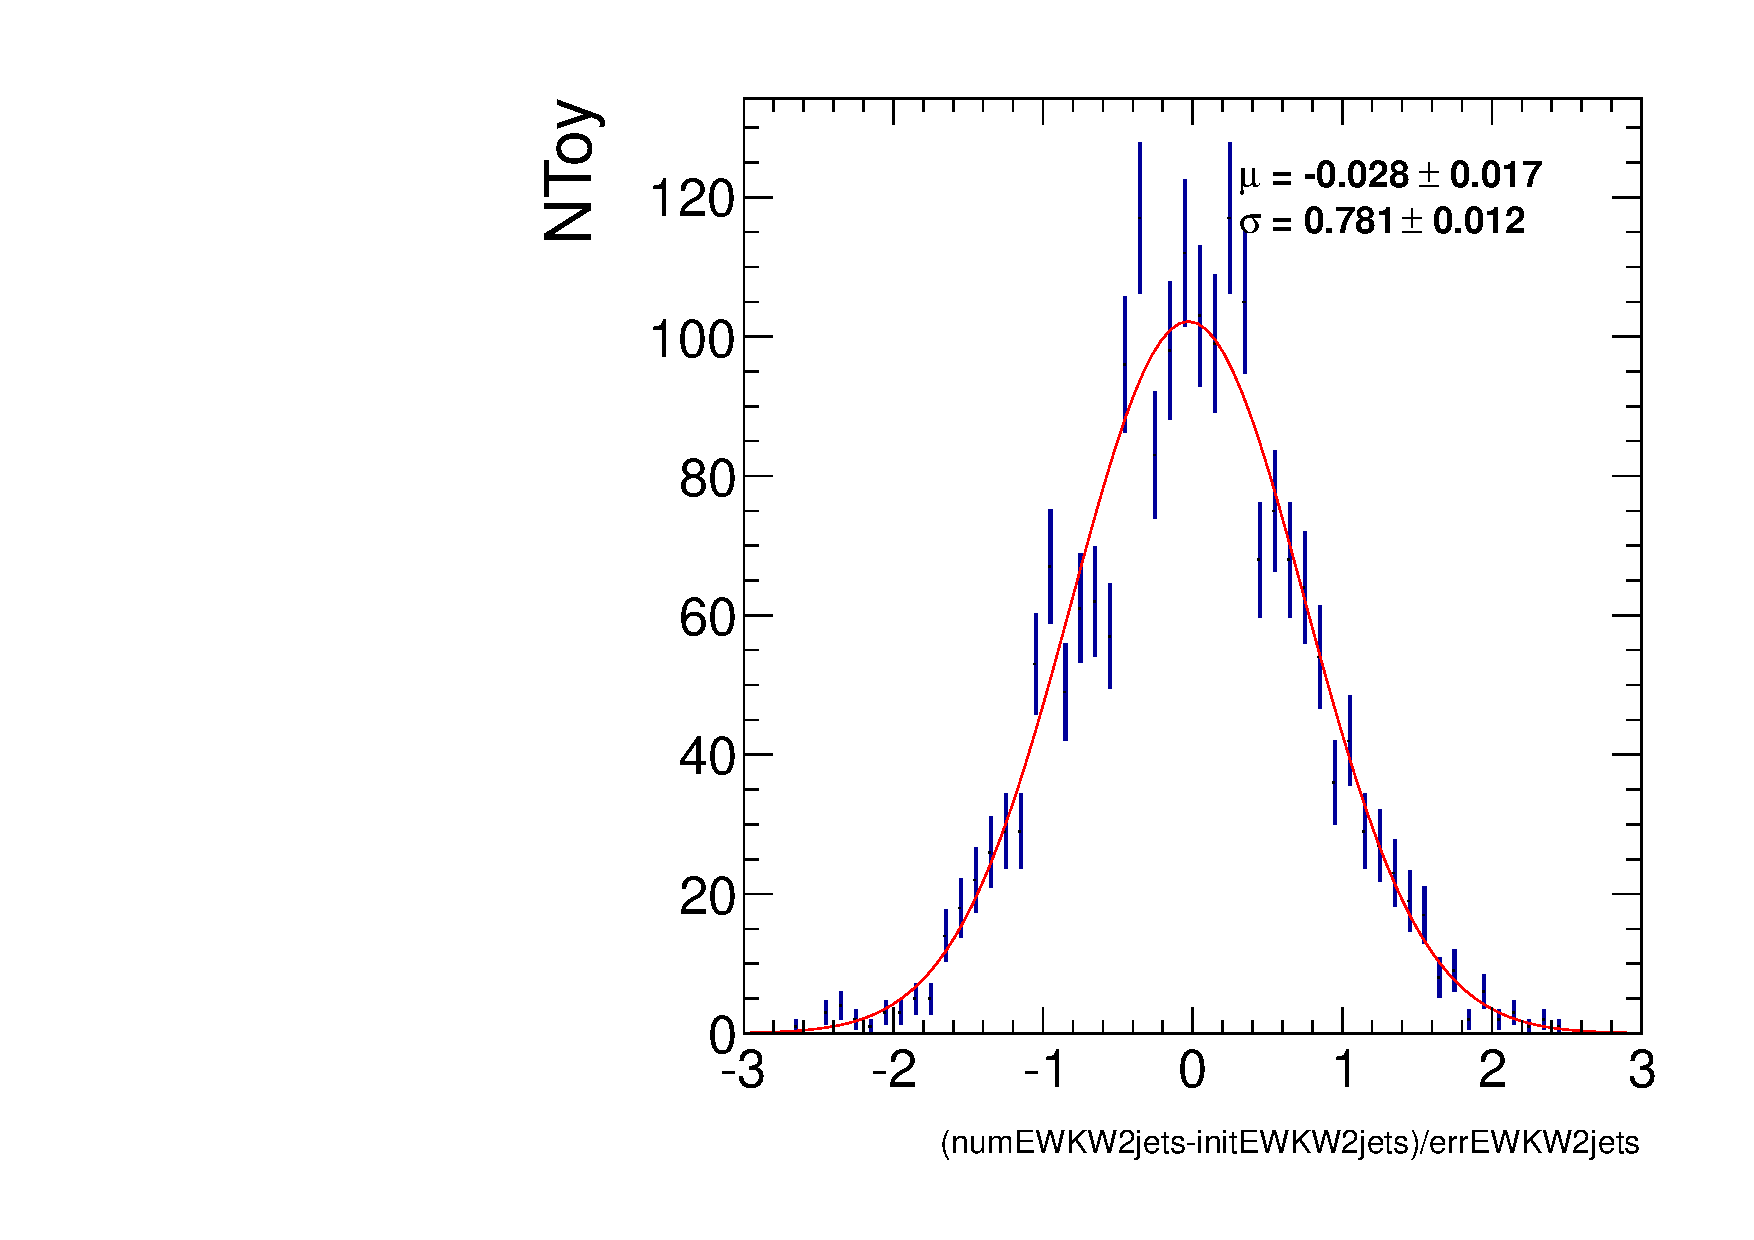
\includegraphics[width=0.48\textwidth]{figs/validation/mu_numEWKW2jets_initEWKW2jets_errEWKW2jets_EWKW2jetspullplot_pulldistribution.pdf}
\put(-0.80,0.0){(b)} \\ 
\unitlength=0.33\linewidth
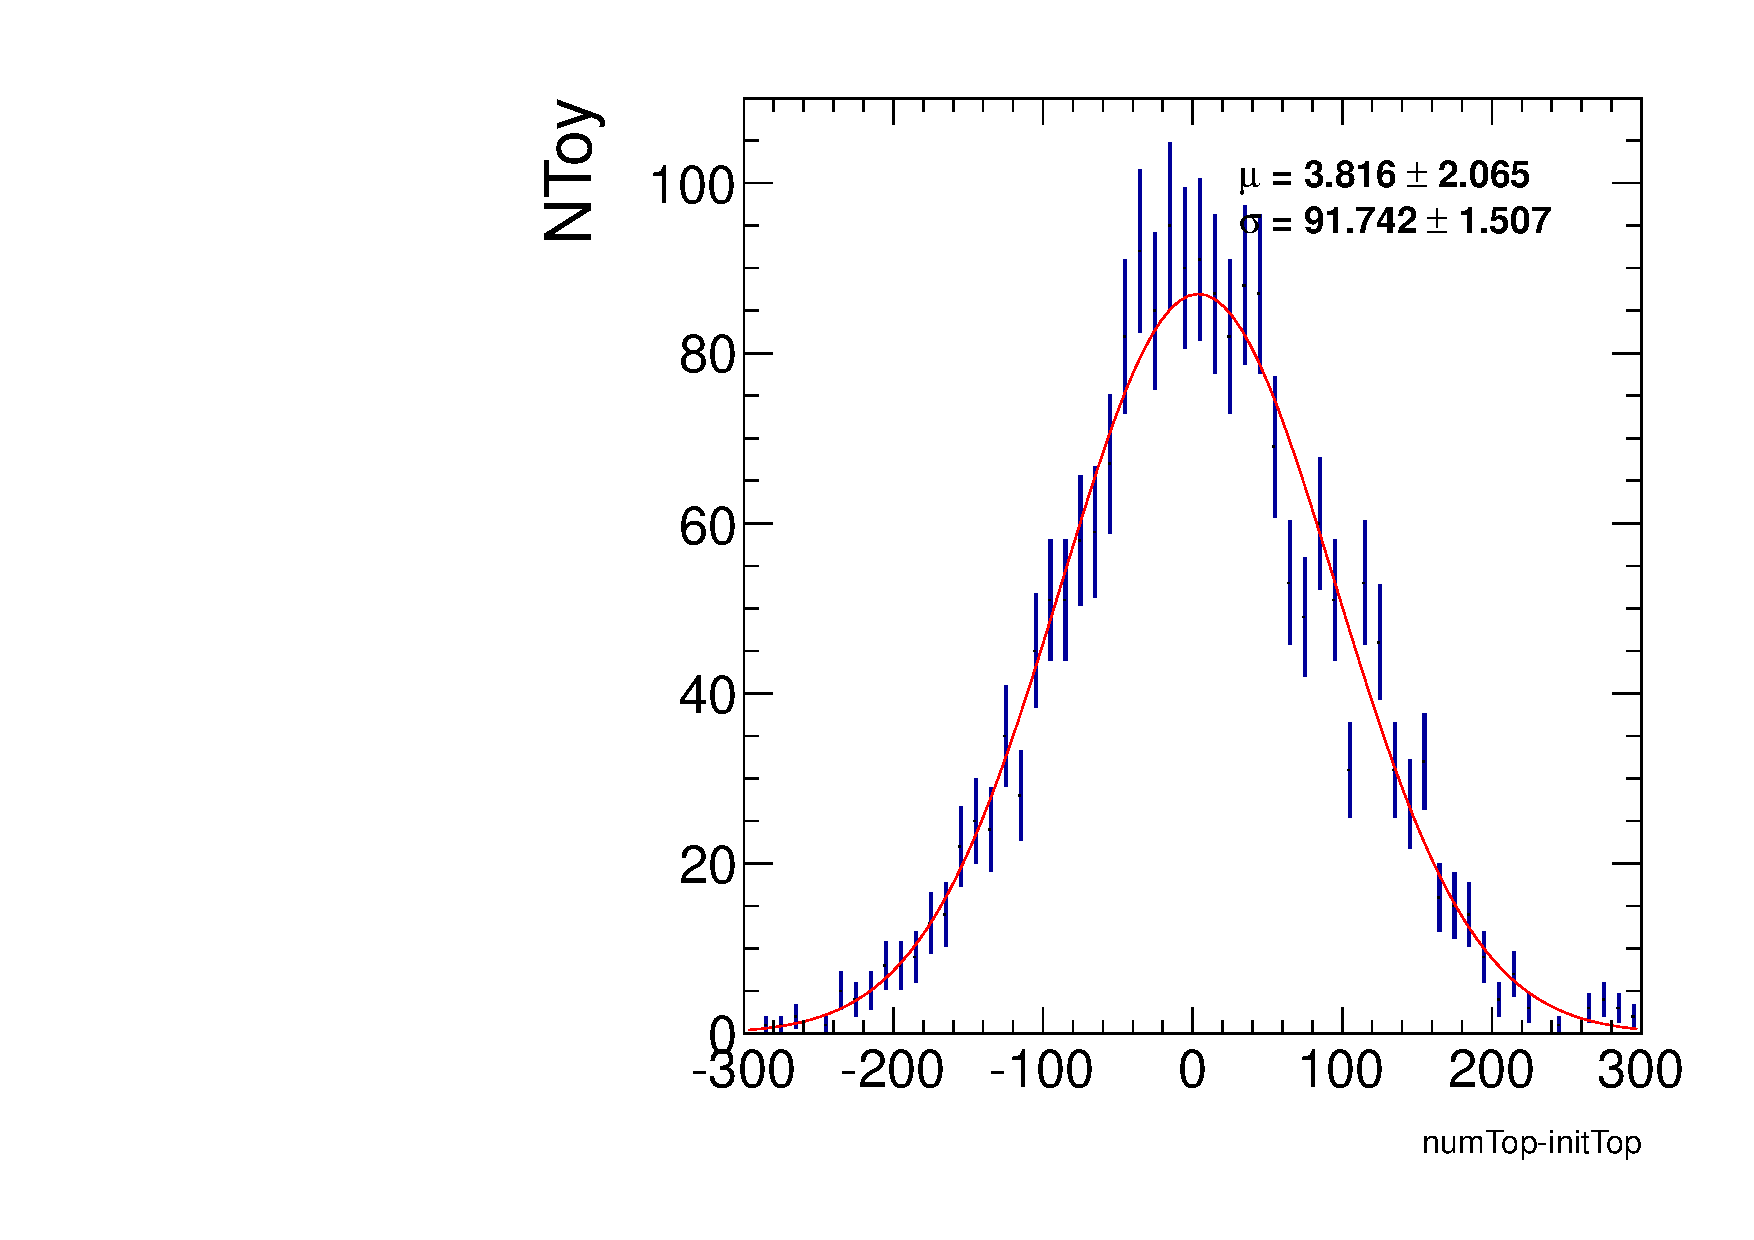
\includegraphics[width=0.48\textwidth]{figs/validation/mu_numTop_initTop_Topbiasplot_pulldistribution.pdf}
\put(-0.80,0.0){(c)}
\unitlength=0.33\linewidth
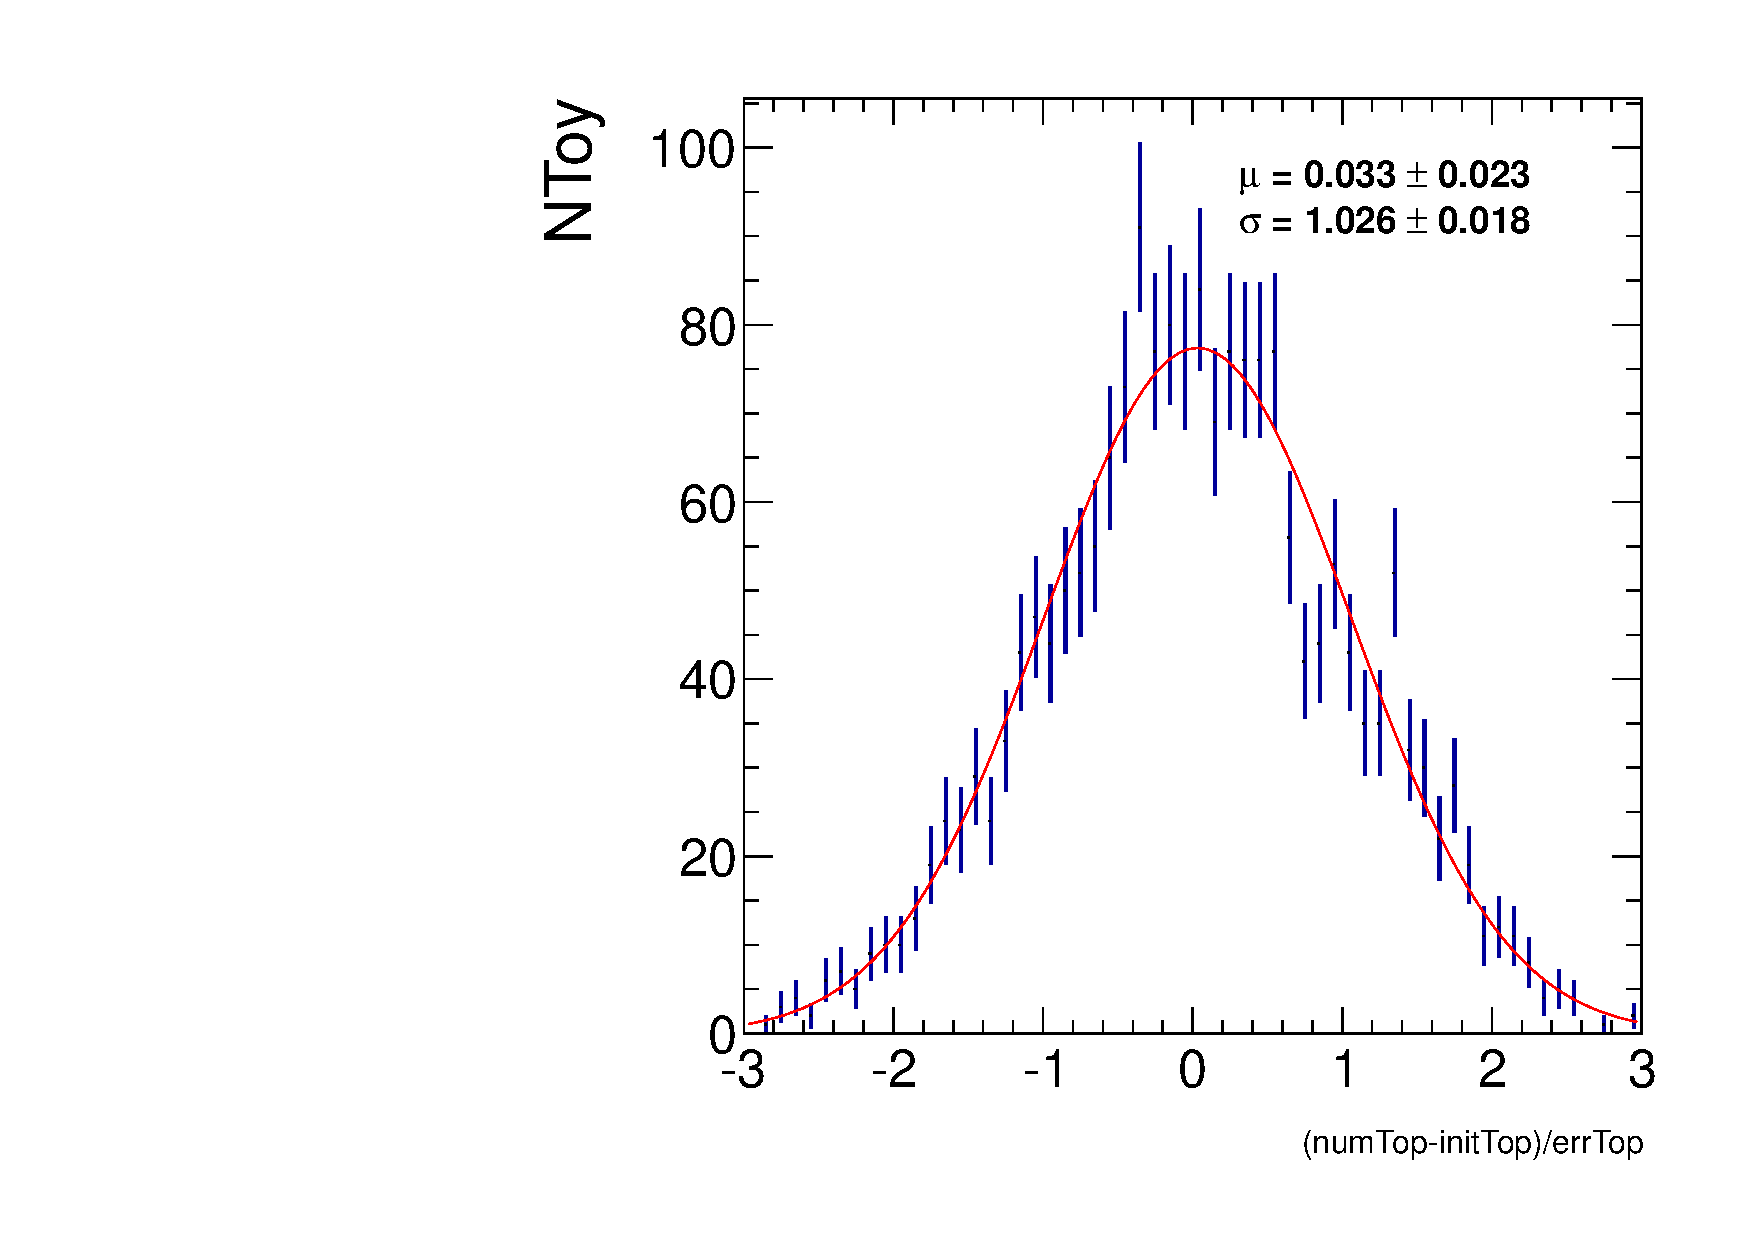
\includegraphics[width=0.48\textwidth]{figs/validation/mu_numTop_initTop_errTop_Toppullplot_pulldistribution.pdf}
\put(-0.80,0.0){(d)} 
\caption{Fit validation in the muon channel, using 2000 Toy MC datasets. Fitted-Given yields for: (a) EWK W+2jets, (c) Top and Pull=(Fitted-Given)/Error for: (b) EWK W+2jets, (d) Top.} 
\label{fig:Validation_mu_Standard}}
\end{figure}
%%%%%%%
%%%%%%%
\begin{figure}[h!] {\centering
\unitlength=0.33\linewidth
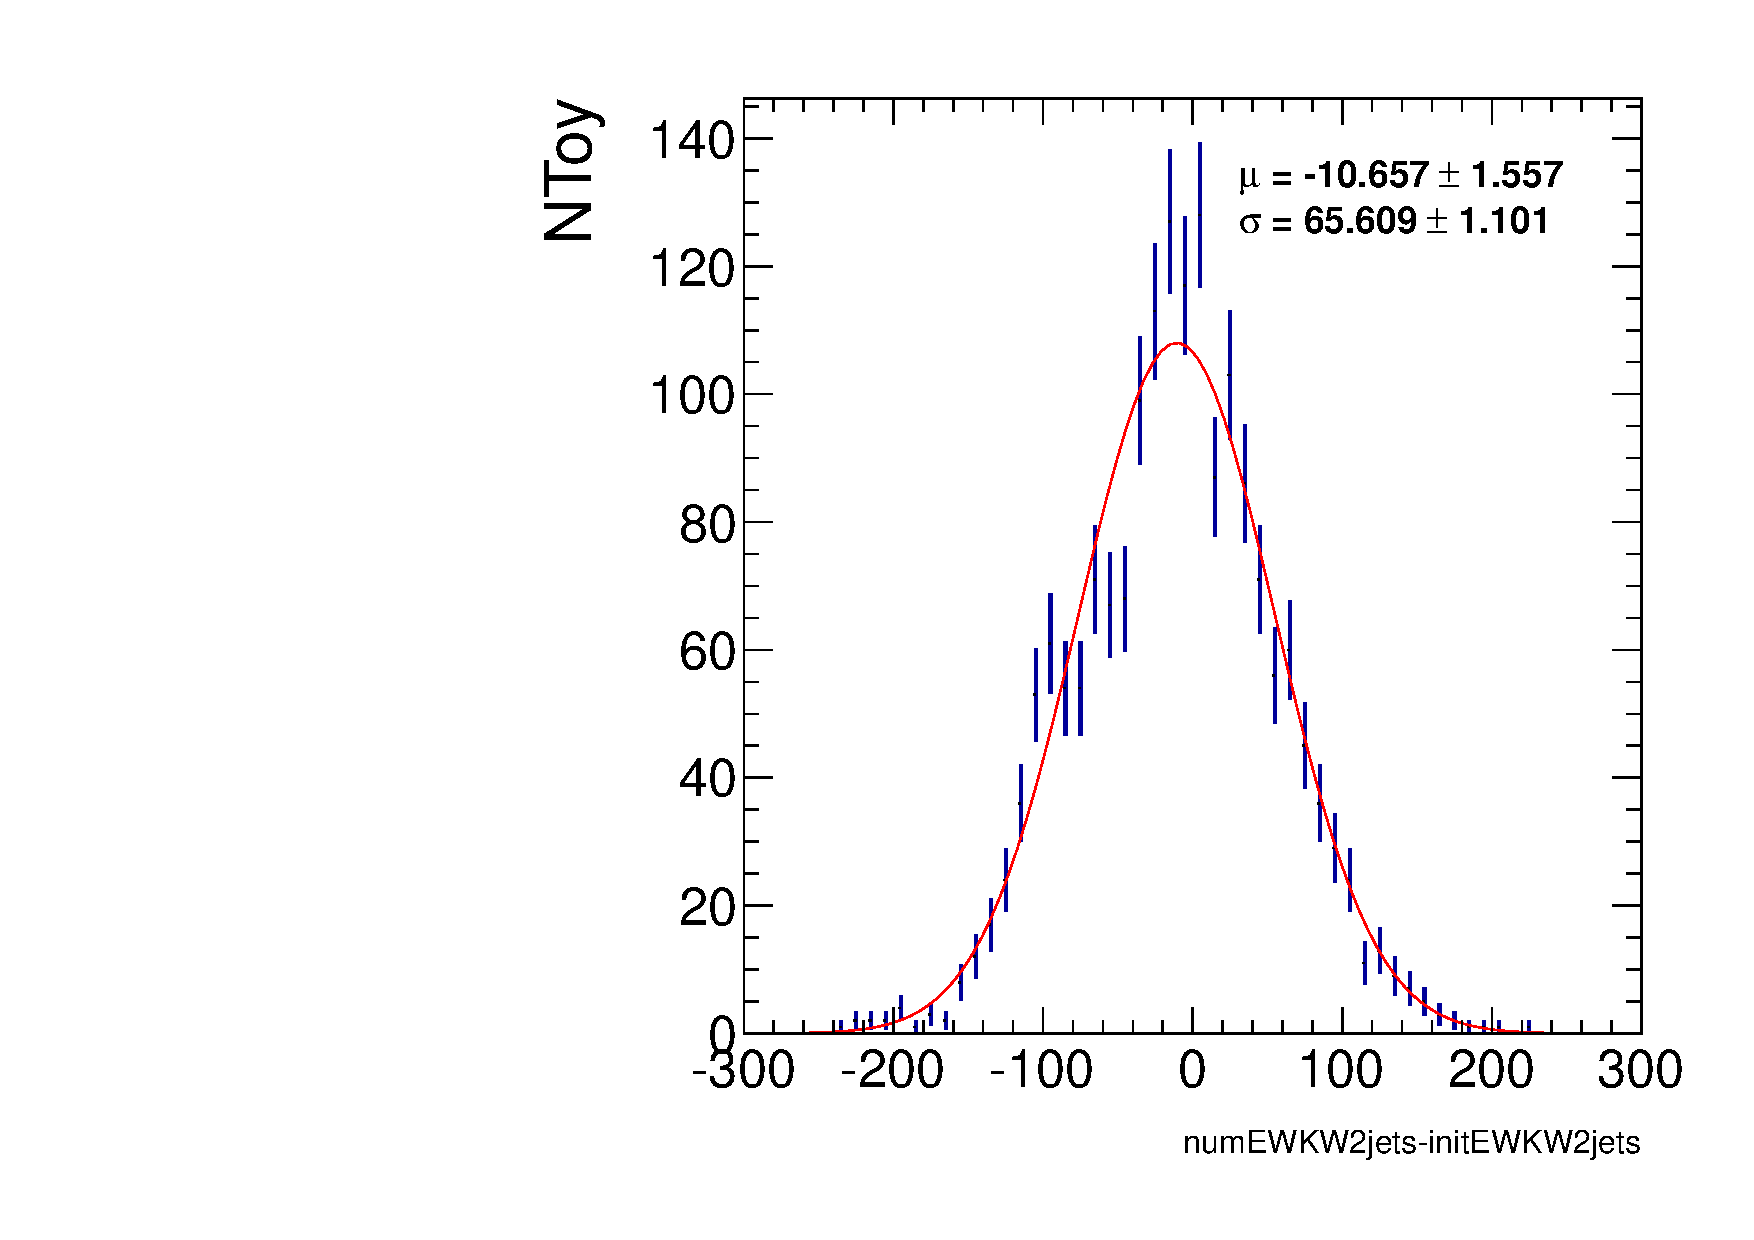
\includegraphics[width=0.48\textwidth]{figs/validation/el_numEWKW2jets_initEWKW2jets_EWKW2jetsbiasplot_pulldistribution.pdf}
\put(-0.80,0.0){(a)}
\unitlength=0.33\linewidth
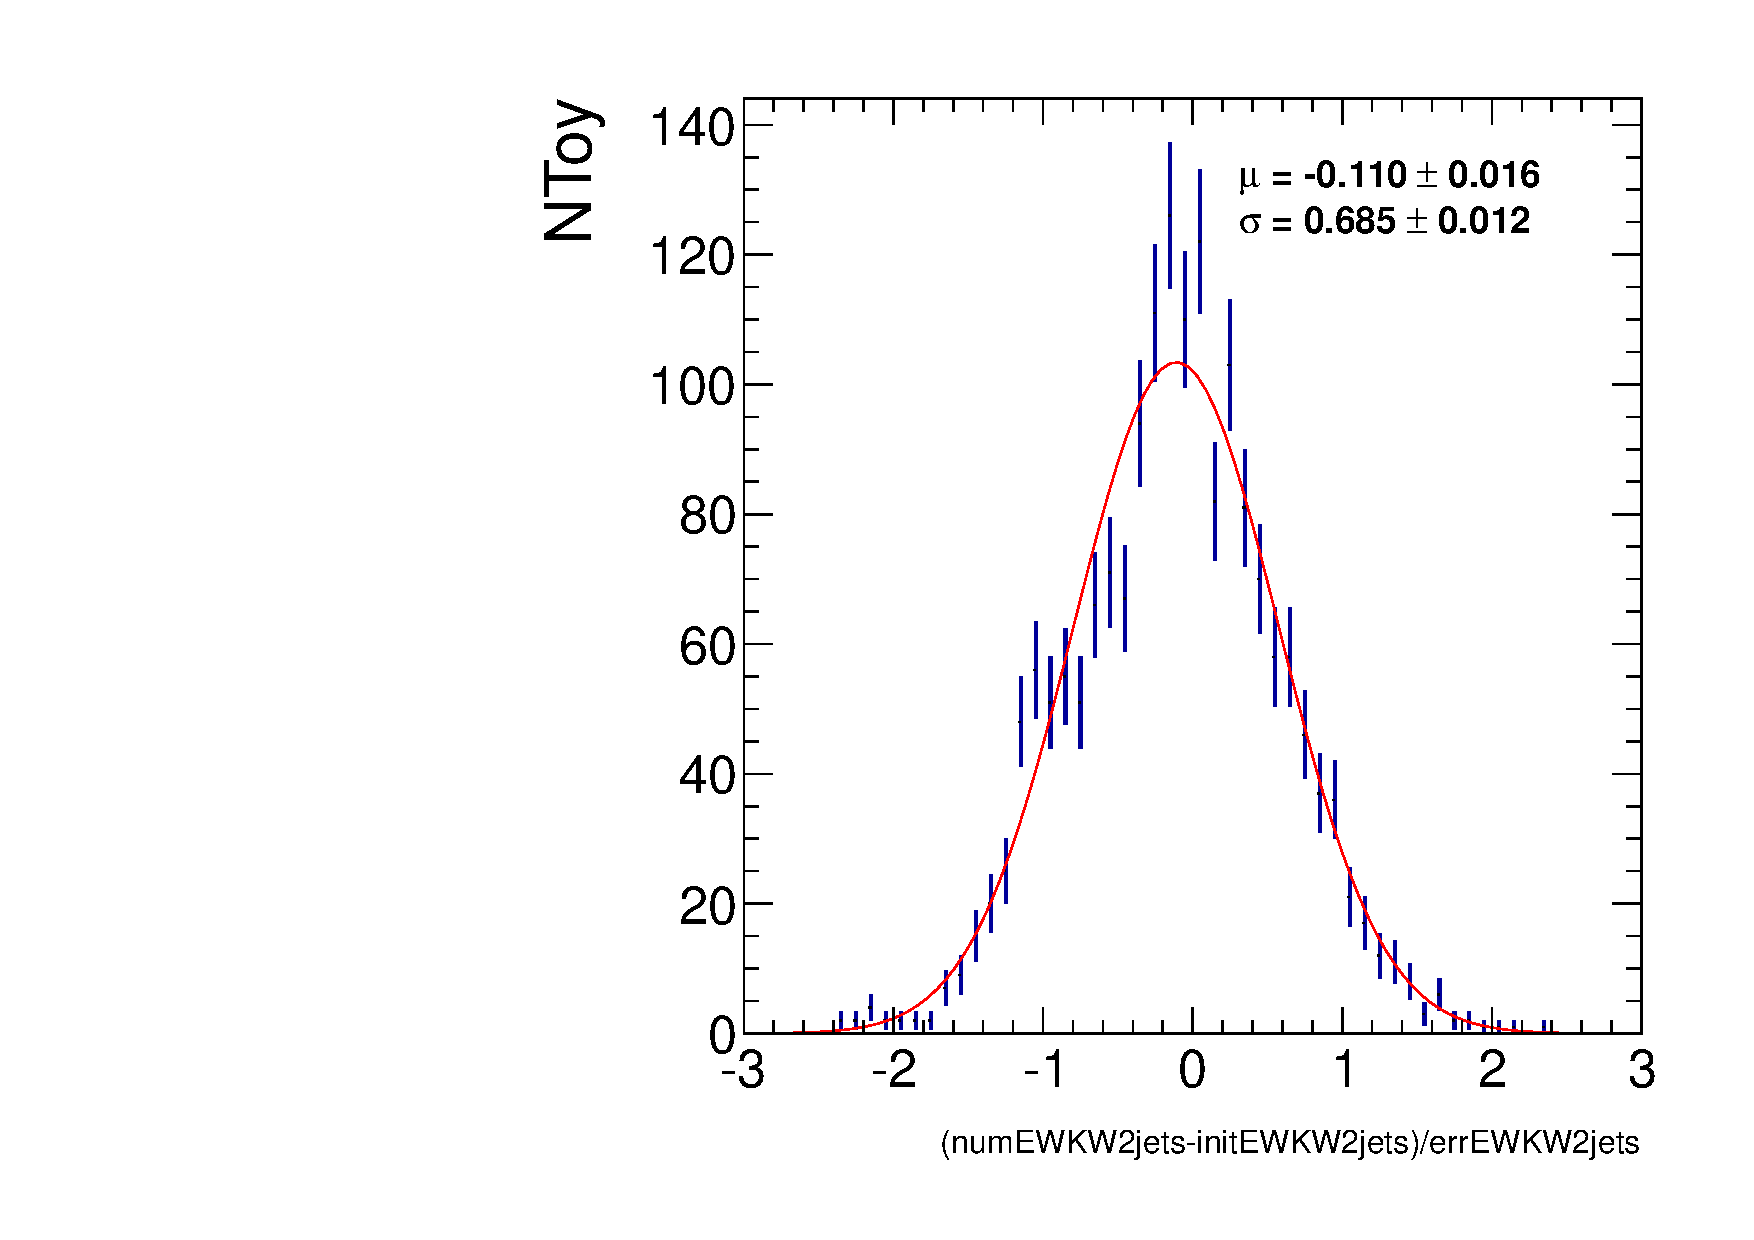
\includegraphics[width=0.48\textwidth]{figs/validation/el_numEWKW2jets_initEWKW2jets_errEWKW2jets_EWKW2jetspullplot_pulldistribution.pdf}
\put(-0.80,0.0){(b)} \\ 
\unitlength=0.33\linewidth
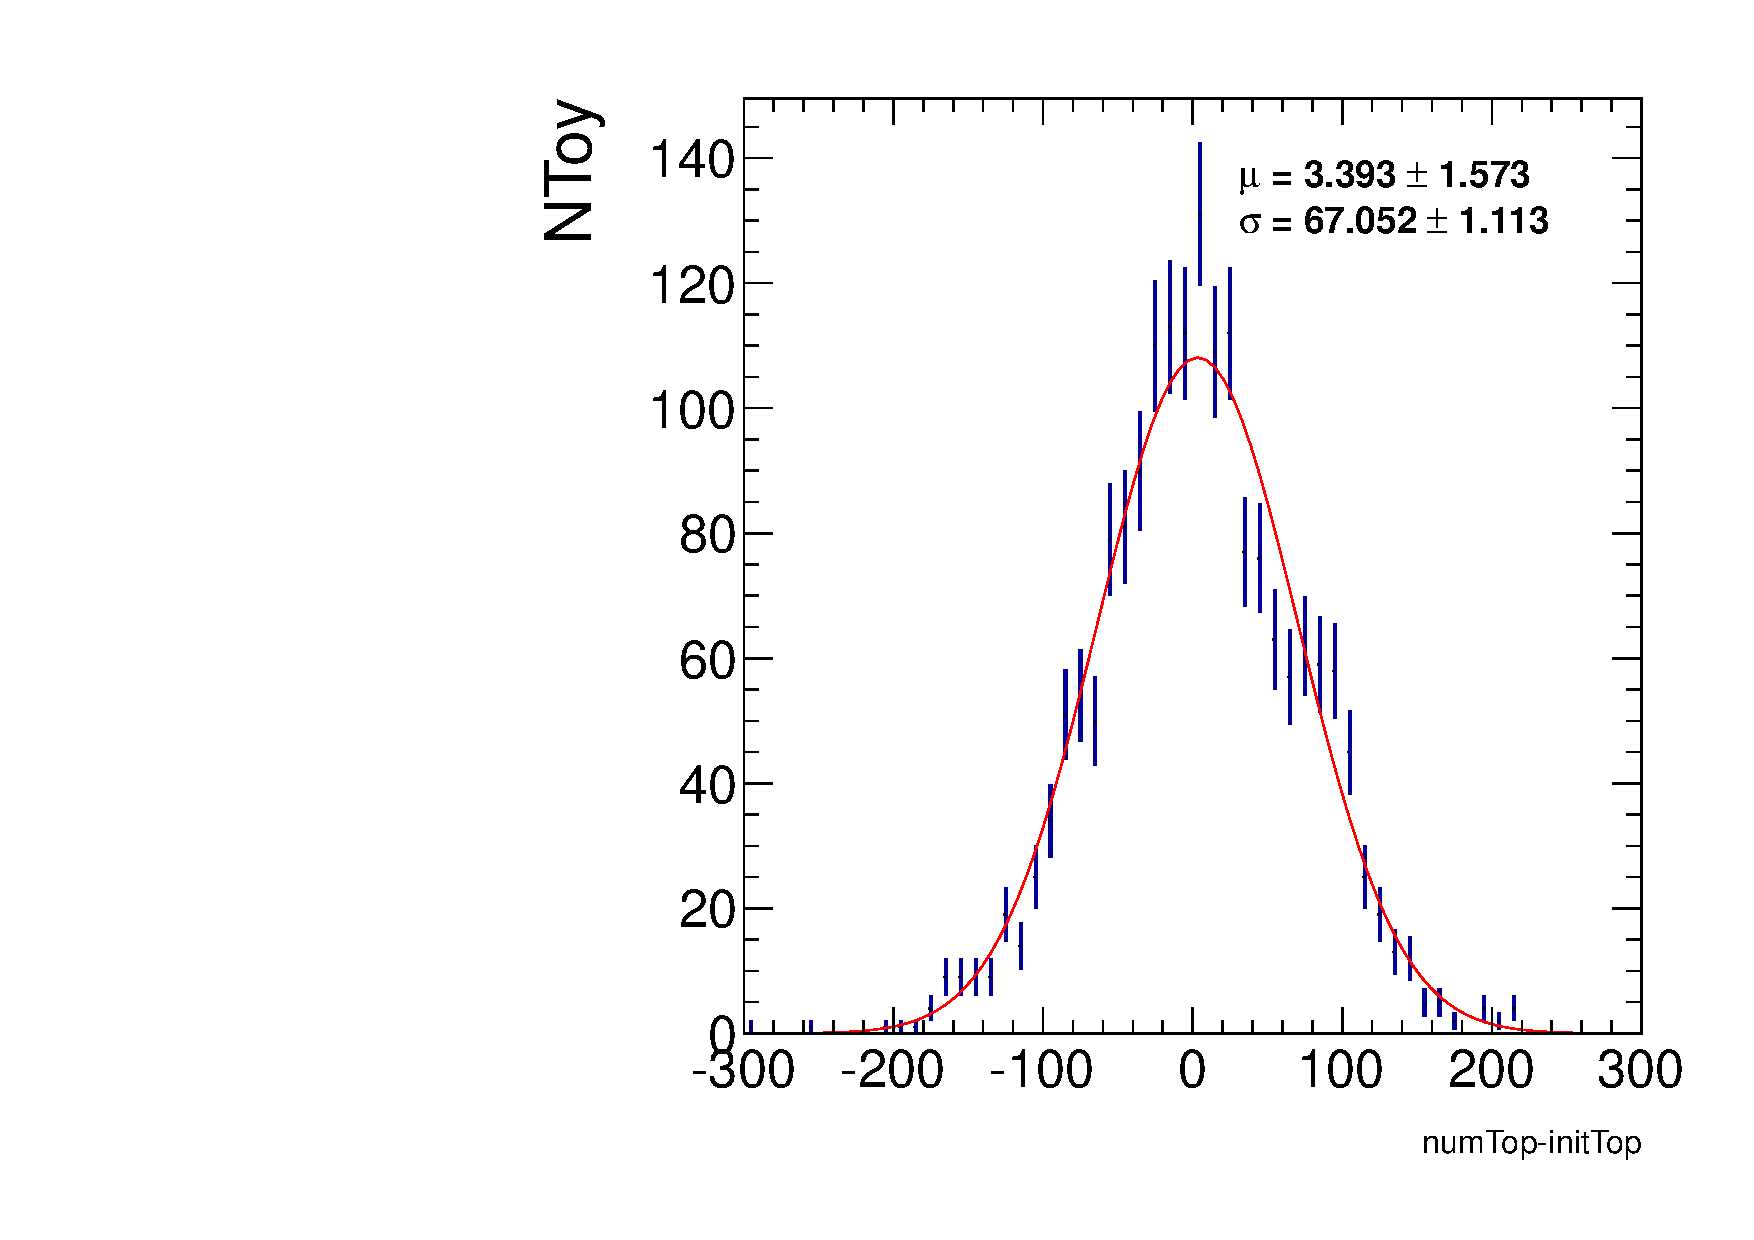
\includegraphics[width=0.48\textwidth]{figs/validation/el_numTop_initTop_Topbiasplot_pulldistribution.pdf}
\put(-0.80,0.0){(c)}
\unitlength=0.33\linewidth
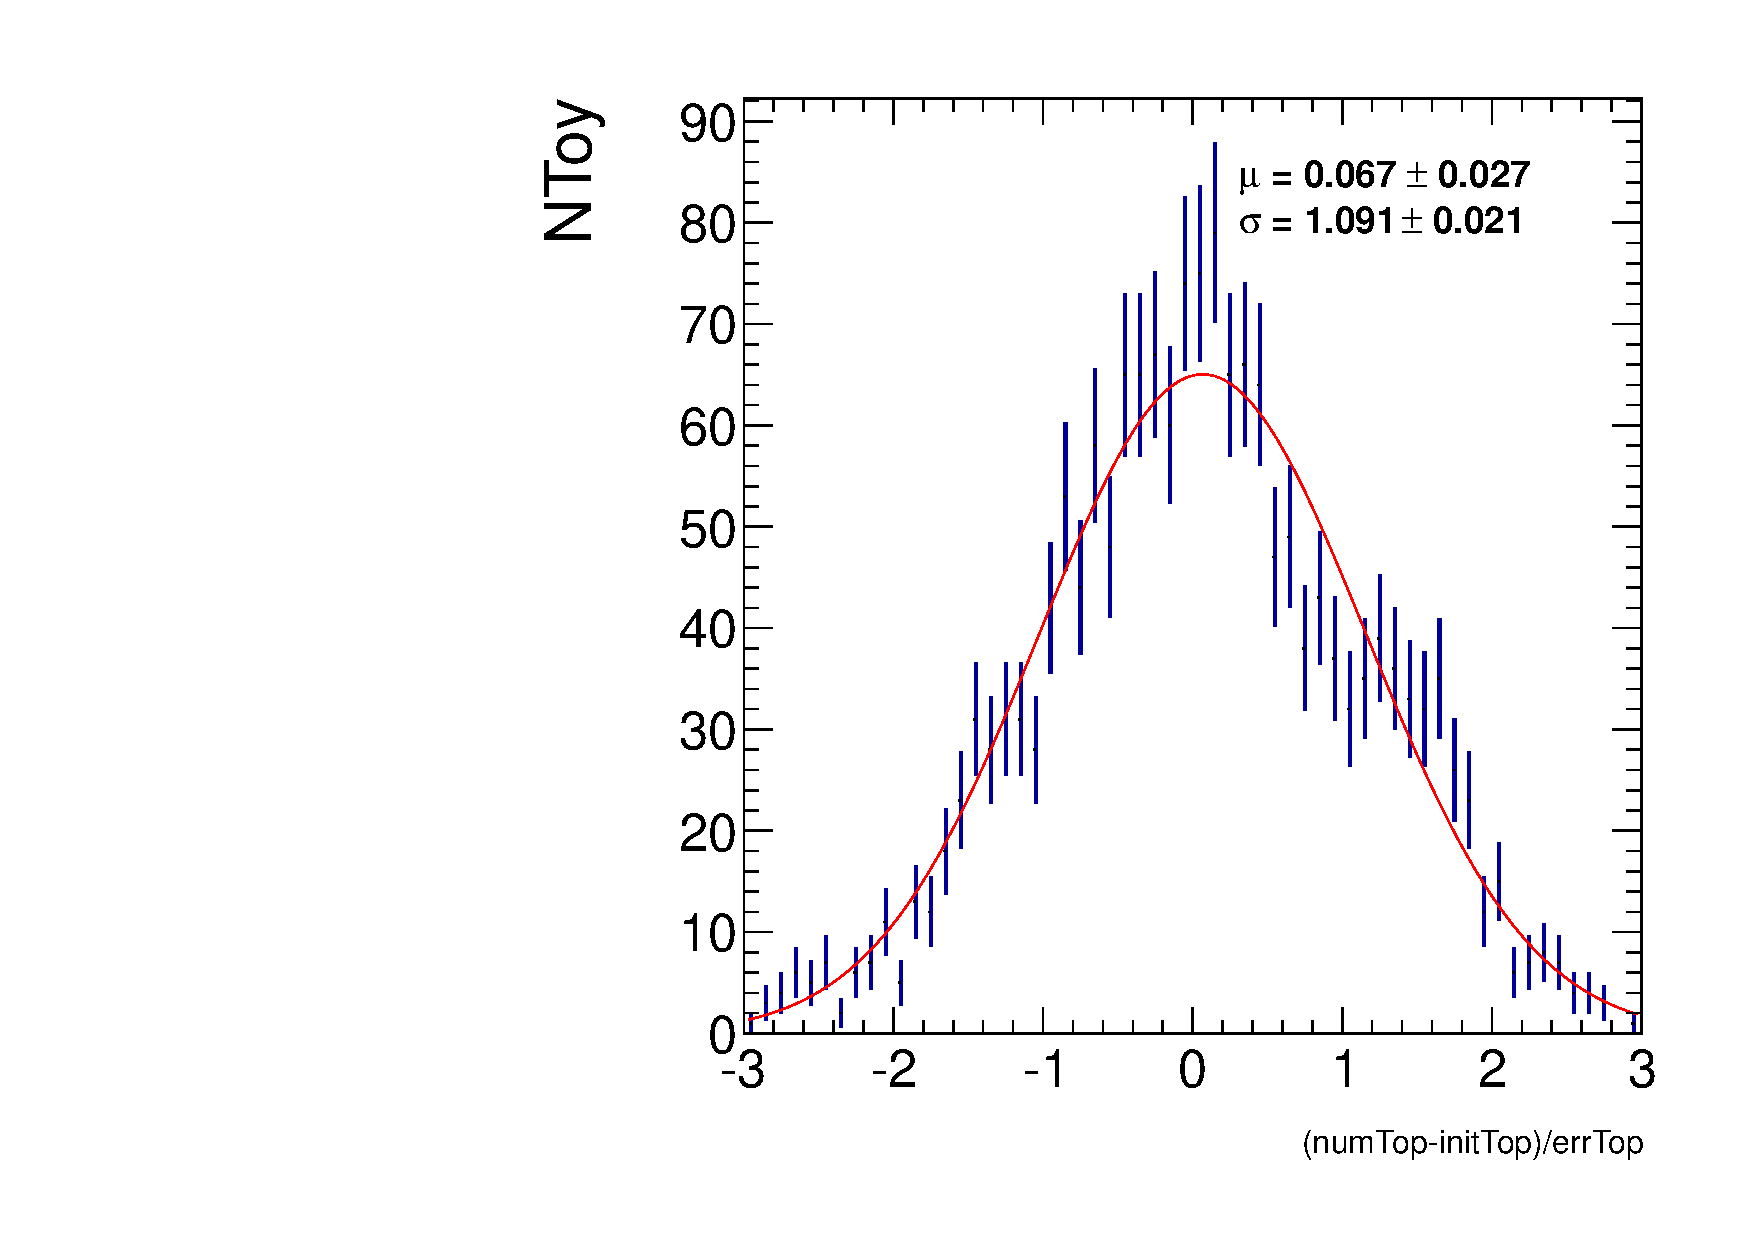
\includegraphics[width=0.48\textwidth]{figs/validation/el_numTop_initTop_errTop_Toppullplot_pulldistribution.pdf}
\put(-0.80,0.0){(d)} 
\caption{Fit validation in the the electron channel, using 2000 Toy MC datasets. Fitted-Given yields for: (a) EWK W+2jets, (c) Top and Pull=(Fitted-Given)/Error for: (b) EWK W+2jets, (d) Top.} 
\label{fig:Validation_el_Standard}}
\end{figure}
%%%%%%%
%%%%%%%%%%%%%%%%%%%%%%%%%

The fit biases for each channel are listed in Table~\ref{tab:SystematicCorrections}. On balance the fit configurations have a minor bias in the yield and overestimate the error by ~20-30\%. This is not unexpected since we do not know the precise parameterization for our background and compensate by using functions which (potentially) have more parameters than, what the 'true' form would contain. Furthermore, the high degree of correlation and similiar falling spectrum between the backgrounds (most notably W+jets) and the electroweak W+2jets impact its uncertainty. We use the above Yield and Pull distributions to correct for these effects in Table~\ref{table:FitCorrectedYields}.

%\subsubsection{Fit Shape Validation}
%Since we are relying on parametric shapes to model the data we need to ensure that the functional form used is sufficiently general and evaluate the corresponding error. First, we use alternate, more general, functional forms to fit the data. Then we generate toy datasets using the alternate form, but with the shape parameters obtained in the fits to the MC (rather than the data) and refit each dataset using the default configuration. {\it I.e.} we ensure that the alternate parametrization produces a good fit to the data, but compare one MC fit result to the other, since the objective is to ascertain the bias strictly due to the shape parameterization (the generated yield values are determined based on the default fit to the data by following the procedure described above). The results are shown in Figs.~\ref{fig:ShapeBias_mu_Standard}.%~\ref{fig:ShapeBias_el_Standard} for the anti-btagged dijet configuration, Figs.~\ref{fig:ShapeBias_mu_Btag},~\ref{fig:ShapeBias_el_Btag} for the btagged dijet configuration and in Figs.~\ref{fig:ShapeBias_mu_Boosted},~\ref{fig:ShapeBias_el_Boosted} for the boosted case.
%
%%%%%%%%%%%%%%%%%%%%%%%%%%
%%%%%%%%
%\begin{figure}[h!] {\centering
%\unitlength=0.33\linewidth
%\includegraphics[width=0.48\textwidth]{figs/validation/.png}
%\put(-0.80,0.0){(a)}
%\unitlength=0.33\linewidth
%\includegraphics[width=0.48\textwidth]{figs/validation/.png}
%\put(-0.80,0.0){(b)} \\ 
%%\unitlength=0.33\linewidth
%%\includegraphics[width=0.48\textwidth]{figs/validation/.png}
%%\put(-0.80,0.0){(c)}
%%\unitlength=0.33\linewidth
%%\includegraphics[width=0.48\textwidth]{figs/validation/.png}
%%\put(-0.80,0.0){(d)} 
%\caption{Shape validation in the muon channel, using 2000 Toy MC datasets. Fitted-Given yields for: (a) W+Jets.} 
%\label{fig:ShapeBias_mu_Standard}}
%\end{figure}
%%%%%%%%
%%%%%%%%
%\begin{figure}[h!] {\centering
%\unitlength=0.33\linewidth
%\includegraphics[width=0.48\textwidth]{figs/validation/.png}
%\put(-0.80,0.0){(a)}
%\unitlength=0.33\linewidth
%\includegraphics[width=0.48\textwidth]{figs/validation/.png}
%\put(-0.80,0.0){(b)} \\ 
%%\unitlength=0.33\linewidth
%%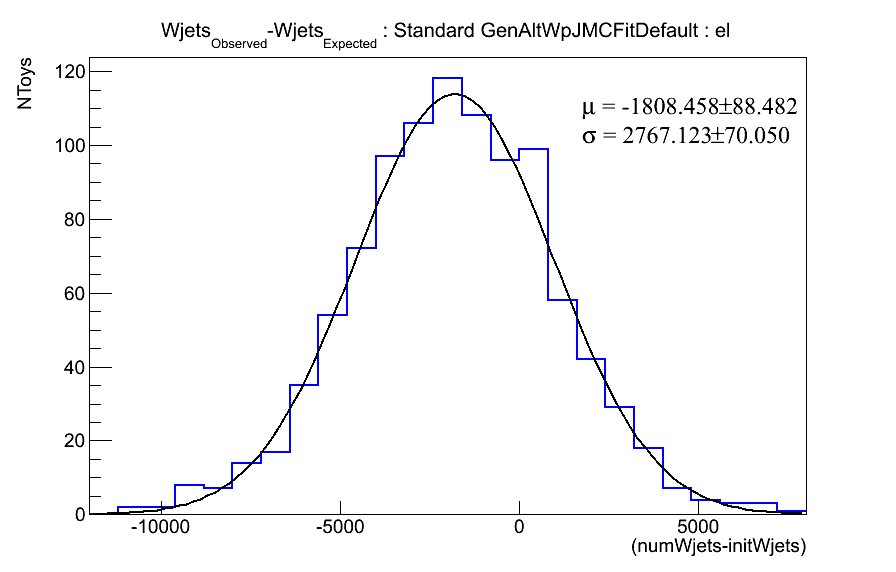
\includegraphics[width=0.48\textwidth]{figs/validation/ShapeBias_WJetsYield_Standard_el.png}
%%\put(-0.80,0.0){(c)}
%%\unitlength=0.33\linewidth
%%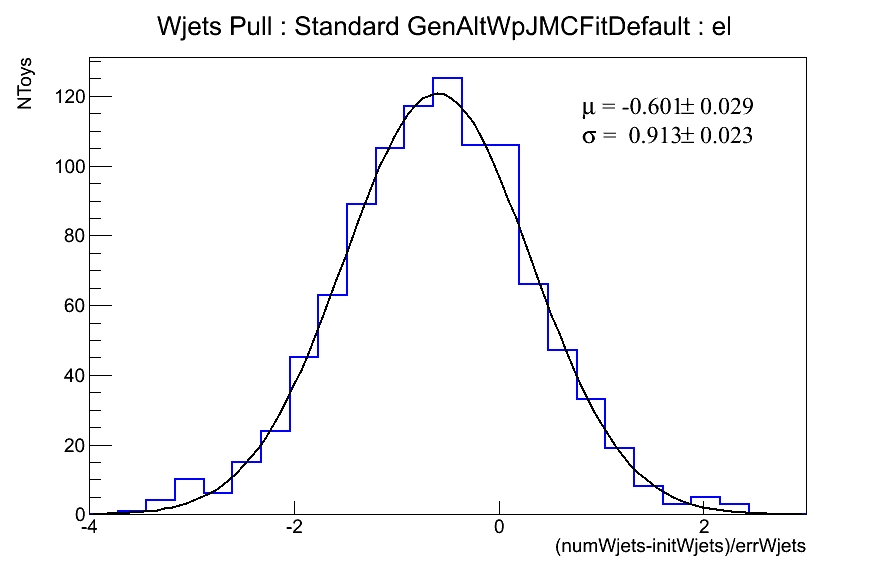
\includegraphics[width=0.48\textwidth]{figs/validation/ShapeBias_WJetsPull_Standard_el.png}
%%\put(-0.80,0.0){(d)} 
%\caption{Shape validation in the the electron channel, using 2000 Toy MC datasets. Fitted-Given yields for: (a) W+Jets.} 
%\label{fig:ShapeBias_el_Standard}}
%\end{figure}
%%%%%%%%%
%
%As can be seen there is an (up to ~20\%) bias between the given and fitted yields. We account for it by adding the offset in the number of events (in quadrature) to the total error. The diboson yields after correcting for (all of) the corresponding biases are listed in Table~\ref{table:FitTotalsAndComparisons}.

%%%%%%%%%%%%%%%%%%%%%%%%%%%%%%%%%%%%%%%%%%%%%%%%%%%%%%%%%%%%
%\subsection{Total Cross Section}
%    Combining the two channels (in Table~\ref{tab:SystematicCorrections}) gives a total of $XXX\pm XXX$ diboson events with a $XXX\sigma$ significance. Upon correcting for biases in the extracted yield and corresponding error as well as shape systematics, we extract XXX $\pm$ XXX (stat) $\pm$ XX (syst) signal events. The electroweak W2jets signal cross section is computed for each of the six channels as $\sigma = N_{\text{Sig}}/ (\mathcal{A} \, \varepsilon \, {\mathcal{L}})$, where $N_{\text{Sig}}$ is the number of extracted signal events, $\mathcal{A}$ is the signal acceptance corrected for the branching fractions, $\varepsilon$ is the overall efficiency for event selection (listed for each channel in Table~\ref{tab:signals}), ${\mathcal{L}}$ is the integrated luminosity. The results are listed in Table~\ref{tab:dibosonYield}. An additional systematic uncertainty (total, without luminosity in Table~\ref{tab:signalSyst}) is added in quadrature to the systematic error. The Luminosity uncertainty (Section~\ref{sec:LumiUncertainty}) is included separately. The total cross section is $XXX\pm XXX\text{(stat)}\pm XXX\text{(syst)}\pm XXX\text{(lumi)}$~pb, statistically consitent with the individual channel results as well as the Standard Model expectation of $XXX\unit{pb}$~\cite{Campbell:2011bn}.
\subsubsection{BDT Output Distribution Signal Region Cross Check Fit}
As a cross check, we directly fit the BDT output distribution in the signal region($>$ 0.1) to calculate the EWK W+2jets signal cross section. In this fit, we fix the W+jets normalization scale factor from the previous W+jets control region fit(BDT $<$ 0.1) and other minor background contributions(ZJets and Diboson). Top(TTbar+SingleTop) and EWK W+2jets signal contributions are float in this fit. This is a cross check result for tagjet pair invariant mass $m_{jj}$ distribution fit. The fit result can be found in Table~\ref{tab:bdtfitresult}. We found consisted fit results between this BDT fit method and tagjet pair invariant mass $m_{jj}$ fit method.

\begin{table}[htb]
\centering
\begin{tabular}{|c|c|c|}
\hline
Channels &  Muons & Electrons \\ \hline
signal strength fit result & 0.956 $\pm$ 0.121(stat.) & 0.826 $\pm$ 0.144(stat.) \\ \hline
\end{tabular}
\caption{EWK W+2jets signal strength fit result in the BDT signal region output distribution fit}
\label{tab:bdtfitresult}
\end{table}

